%%%%%%%%%%%%%%%%%%%%%%%%%%%%%%%%%%%%%%%%%%%%%%%%%%%%%%%%%%%%%%%%%%%%%%%%%%%
%% This file is part of the book
%%
%% Algorithmic Graph Theory
%% http://code.google.com/p/graph-theory-algorithms-book/
%%
%% Copyright (C) 2010 David Joyner <wdjoyner@gmail.com>
%% Copyright (C) 2009, 2010, 2011 Minh Van Nguyen <nguyenminh2@gmail.com>
%%
%% See the file COPYING for copying conditions.
%%%%%%%%%%%%%%%%%%%%%%%%%%%%%%%%%%%%%%%%%%%%%%%%%%%%%%%%%%%%%%%%%%%%%%%%%%%

\chapter{Trees and Forests}
\label{chap:trees_forests}

\begin{quote}
\footnotesize
\includegraphics[scale=3]{image/trees-forests/in-the-trees.png} \\
\noindent
--- Randall Munroe\index{Munroe, Randall}, xkcd,
\url{http://xkcd.com/71/}
\end{quote}

\noindent
In section~\ref{subsec:introduction:walks_trails_paths}, we briefly
touched upon trees\index{tree} and provided examples of how trees
could be used to model hierarchical\index{hierarchical structure}
structures. This chapter provides an in-depth study of
trees\index{tree}, their properties, and various applications. After
defining trees and related concepts in
section~\ref{sec:trees_forests:definitions_examples}, we then present
various basic properties of trees in
section~\ref{sec:trees_forests:properties_trees}. Each connected graph
$G$ has an underlying subgraph called a spanning tree that contains
all the vertices of $G$. Spanning trees are discussed in
section~\ref{sec:trees_forests:minimum_spanning_trees} together with
various common algorithms for finding spanning trees. We then discuss
binary trees in section~\ref{sec:trees_forests:binary_trees}, followed
by an application of binary trees to coding theory in
section~\ref{sec:trees_forests:Huffman_codes}. Whereas breadth- and
depth-first searches are general methods for traversing a graph, trees
require specialized techniques in order to visit their vertices, a
topic that is taken up in section~\ref{sec:trees_forests:tree_traversals}.


%%%%%%%%%%%%%%%%%%%%%%%%%%%%%%%%%%%%%%%%%%%%%%%%%%%%%%%%%%%%%%%%%%%%%%%%%%%

\section{Definitions and examples}
\label{sec:trees_forests:definitions_examples}

\begin{quote}
\footnotesize
I think that I shall never see \\
A poem lovely as a tree. \\
\noindent
--- Joyce Kilmer, \emph{Trees and Other Poems}, 1914, ``Trees''
\end{quote}

\noindent
Recall that a path\index{path} in a graph $G = (V, E)$ whose start and
end vertices are the same is called a cycle\index{cycle}. We say $G$ is
\emph{acyclic}\index{acyclic}, or a \emph{forest}\index{forest}, if it
has no cycles. In a forest, a vertex of degree one is called an
\emph{endpoint}\index{vertex!endpoint} or a
\emph{leaf}\index{vertex!leaf}. Any vertex that is not a
leaf\index{vertex!leaf} is called an \emph{internal} vertex. A
connected forest\index{forest} is a \emph{tree}\index{tree}. In other
words, a tree\index{tree} is a graph without cycles\index{cycle} and
each edge is a bridge\index{bridge}. A forest can also be considered
as a collection of trees.

A \emph{rooted tree}\index{tree!rooted} $T$ is a tree\index{tree} with
a specified \emph{root}\index{vertex!root} vertex $v_0$, i.e. exactly
one vertex has been specially designated as the root of $T$. However,
if $G$ is a rooted\index{tree!rooted} tree with root vertex $v_0$
having degree one, then by convention we do not call $v_0$ an
endpoint\index{vertex!endpoint} or a leaf\index{vertex!leaf}. The
\emph{depth}\index{tree!depth}\index{tree!depth}
$\depth(v)$\index{$\depth(v)$} of a vertex $v$ in $T$ is its
distance\index{distance} from the
root\index{vertex!root}. The \emph{height}\index{tree!height}
$\height(T)$\index{$\height(T)$} of $T$ is the
length\index{path!length} of a longest path\index{path} starting from
the root\index{vertex!root} vertex, i.e. the height\index{tree!height}
is the maximum depth\index{tree!depth} among all vertices of $T$. It
follows by definition that $\depth(v) = 0$\index{tree!depth} if and
only if $v$ is the root of $T$, $\height(T) = 0$\index{tree!height} if
and only if $T$ is the trivial\index{trivial graph} graph,
$\depth(v) \geq 0$\index{tree!depth} for all $v \in V(T)$, and
$\height(T) \leq \diam(T)$\index{tree!height}.

The Unix\index{Unix}, in particular Linux\index{Linux},
filesystem\index{filesystem} hierarchy\index{hierarchical structure}
can be viewed as a tree~(see
Figure~\ref{fig:trees_forests:filesystem_hierarchy}). As shown in
Figure~\ref{fig:trees_forests:filesystem_hierarchy}, the
root\index{vertex!root} vertex is designated with the forward slash,
which is also referred to as the root
directory\index{root directory}. Other examples of trees include the
organism classification\index{classification tree} tree in
Figure~\ref{fig:trees_forests:classification_tree_organisms}, the
family\index{family tree} tree in
Figure~\ref{fig:trees_forests:Bernoulli_family_tree}, and the
expression\index{tree!expression} tree in
Figure~\ref{fig:trees_forests:expression_tree_perfect_square}.

A \emph{directed tree}\index{tree!directed} is a
digraph\index{digraph} which would be a tree if the directions on the
edges were ignored. A rooted\index{tree!rooted} tree can be regarded
as a directed\index{tree!directed} tree since we can imagine an edge
$uv$ for $u,v \in V$ being directed from $u$ to $v$ if and only if $v$ is
further away from $v_0$ than $u$ is. If $uv$ is an edge in a
rooted\index{tree!rooted} tree, then we call $v$ a
\emph{child}\index{vertex!child} vertex with
\emph{parent}\index{vertex!parent} $u$. Directed\index{tree!directed}
trees are pervasive in theoretical computer science, as they are
useful structures for describing algorithms and relationships between
objects in certain datasets.

\begin{figure}[!htbp]
\centering
\index{filesystem!hierarchy}
\index{Linux}
\includegraphics{image/trees-forests/filesystem-hierarchy}
\caption{The Linux filesystem hierarchy.}
\label{fig:trees_forests:filesystem_hierarchy}
\end{figure}

\begin{figure}[!htbp]
\centering
\index{organism}
\index{classification tree}
\includegraphics{image/trees-forests/classification-tree-organisms}
\caption{Classification tree of organisms.}
\label{fig:trees_forests:classification_tree_organisms}
\end{figure}

\begin{figure}[!htbp]
\centering
\index{Bernoulli family}
\index{family tree}
\includegraphics{image/trees-forests/Bernoulli-family-tree}
\caption{Bernoulli family tree of mathematicians.}
\label{fig:trees_forests:Bernoulli_family_tree}
\end{figure}

\begin{figure}[!htbp]
\centering
\index{perfect square}
\index{tree!expression}
\includegraphics{image/trees-forests/expression-tree-perfect-square}
\caption{Expression tree for the perfect square $a^2 + 2ab + b^2$.}
\label{fig:trees_forests:expression_tree_perfect_square}
\end{figure}

An \emph{ordered tree}\index{tree!ordered} is a
rooted\index{tree!rooted} tree for which an ordering is specified for
the children\index{vertex!child} of each vertex. An
$n$-\emph{ary tree}\index{tree!$n$-ary} is a rooted tree for which
each vertex that is not a leaf\index{vertex!leaf} has at most $n$
children. The case $n = 2$ are called
\emph{binary trees}\index{tree!binary}. An $n$-ary\index{tree!$n$-ary}
tree is said to be \emph{complete}\index{tree!complete} if each of its
internal\index{vertex!internal} vertices has exactly $n$
children\index{vertex!child} and all leaves\index{vertex!leaf} have
the same depth\index{tree!depth}\index{tree!depth}. A
\emph{spanning tree}\index{spanning tree} of a connected, undirected
graph $G$ is a subgraph that is a tree and containing all vertices of
$G$.

\begin{example}
\label{eg:trees_forests:spanning_tree}
{\rm
Consider the $4 \times 4$ grid\index{grid!graph} graph with $16$
vertices and $24$ edges. Two examples of a
spanning\index{spanning tree} tree are given in
Figure~\ref{fig:trees_forests:grid_graph_spanning_trees} by using a
darker line shading for its edges.}
\qed
\end{example}

\begin{figure}[!htbp]
\centering
\index{grid!graph}
\index{spanning tree}
\subfigure[]{
  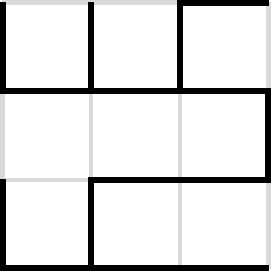
\includegraphics{image/trees-forests/grid-graph-spanning-trees_a}
}
\qquad
\subfigure[]{
  \includegraphics{image/trees-forests/grid-graph-spanning-trees_b}
}
\caption{Two spanning trees for the $4 \times 4$ grid graph.}
\label{fig:trees_forests:grid_graph_spanning_trees}
\end{figure}

\begin{example}
For $n = 1, \dots, 6$, how many distinct
(nonisomorphic)\index{tree!nonisomorphic} trees are there of order
$n$? Construct all such trees for each $n$.
\end{example}

\begin{proof}[Solution]
For $n = 1$, there is only one tree of order $1$, i.e. $K_1$. The same
is true for $n = 2$ and $n = 3$, where the required trees are $P_2$
and $P_3$, respectively (see
Figure~\ref{fig:trees_forests:distinct_trees_specified_order_1_2_3}). We
have two trees of order $n = 4$ (see
Figure~\ref{fig:trees_forests:distinct_trees_specified_order_4}),
three of order $n = 5$ (see
Figure~\ref{fig:trees_forests:distinct_trees_specified_order_5}), and
six of order $n = 6$ (see
Figure~\ref{fig:trees_forests:distinct_trees_specified_order_6}).
\end{proof}

\begin{figure}[!htbp]
\centering
\index{tree!nonisomorphic}
\subfigure[$n = 1$]{
  \includegraphics{image/trees-forests/distinct-trees-specified-order-1-2-3_n1}
}
\quad
\subfigure[$n = 2$]{
  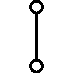
\includegraphics{image/trees-forests/distinct-trees-specified-order-1-2-3_n2}
}
\quad
\subfigure[$n = 3$]{
  \includegraphics{image/trees-forests/distinct-trees-specified-order-1-2-3_n3}
}
\caption{All distinct trees of order $n = 1, 2, 3$.}
\label{fig:trees_forests:distinct_trees_specified_order_1_2_3}
\end{figure}

\begin{figure}[!htbp]
\centering
\index{tree!nonisomorphic}
\subfigure[]{
  \includegraphics{image/trees-forests/distinct-trees-specified-order-4_line}
}
\quad
\subfigure[]{
  \includegraphics{image/trees-forests/distinct-trees-specified-order-4_star}
}
\caption{All distinct trees of order $n = 4$.}
\label{fig:trees_forests:distinct_trees_specified_order_4}
\end{figure}

\begin{figure}[!htbp]
\centering
\index{tree!nonisomorphic}
\subfigure[]{
  \includegraphics{image/trees-forests/distinct-trees-specified-order-5_a}
}
\quad
\subfigure[]{
  \includegraphics{image/trees-forests/distinct-trees-specified-order-5_b}
}
\quad
\subfigure[]{
  \includegraphics{image/trees-forests/distinct-trees-specified-order-5_c}
}
\caption{All distinct trees of order $n = 5$.}
\label{fig:trees_forests:distinct_trees_specified_order_5}
\end{figure}

\begin{figure}[!htbp]
\centering
\index{tree!nonisomorphic}
\subfigure[]{
  \includegraphics{image/trees-forests/distinct-trees-specified-order-6_a}
}
\quad
\subfigure[]{
  \includegraphics{image/trees-forests/distinct-trees-specified-order-6_b}
}
\quad
\subfigure[]{
  \includegraphics{image/trees-forests/distinct-trees-specified-order-6_c}
}
\quad
\subfigure[]{
  \includegraphics{image/trees-forests/distinct-trees-specified-order-6_d}
}
\quad
\subfigure[]{
  \includegraphics{image/trees-forests/distinct-trees-specified-order-6_e}
}
\quad
\subfigure[]{
  \includegraphics{image/trees-forests/distinct-trees-specified-order-6_f}
}
\caption{All distinct trees of order $n = 6$.}
\label{fig:trees_forests:distinct_trees_specified_order_6}
\end{figure}

\begin{example}
\label{eg:trees_forests:branch_cut_binary_tree}
Let $T = (V, E)$ be a tree with vertex set
\[
V
=
\{a, b, c, d, e, f, v, w, x, y, z\}
\]
edge set
\[
E
=
\{va,\, vw,\, wx,\, wy,\, xb,\, xc,\, yd,\, yz,\, ze,\, zf\}
\]
and root vertex $v$. Verify that $T$ is a binary\index{binary tree}
tree. Suppose that $x$ is the root\index{vertex!root} of the branch we
want to remove from $T$. Find all children of $x$ and
cut\index{branch cut} off the branch rooted at $x$ from $T$. Is the
resulting graph also a binary tree?
\end{example}

\begin{proof}[Solution]
We construct the tree $T$ in Sage as follows:
%%
\begin{lstlisting}
sage: T = DiGraph({
...   "v":["a","w"], "w":["x","y"],
...   "x":["c","b"], "y":["z","d"],
...   "z":["f","e"]})
sage: for v in T.vertex_iterator():
...       print(v),
a c b e d f w v y x z
sage: for e in T.edge_iterator():
...       print("%s%s" % (e[0], e[1])),
wy wx va vw yd yz xc xb ze zf
\end{lstlisting}
%%
Each vertex in a binary\index{binary tree} tree has at most $2$
children\index{vertex!child}. Use this definition to test whether or
not a graph is a binary\index{binary tree} tree.
%%
\begin{lstlisting}
sage: T.is_tree()
True
sage: def is_bintree1(G):
...       for v in G.vertex_iterator():
...           if len(G.neighbors_out(v)) > 2:
...               return False
...       return True
sage: is_bintree1(T)
True
\end{lstlisting}
%%
Here's another way to test for binary\index{binary tree} trees. Let
$T$ be an undirected rooted\index{tree!rooted} tree. Each vertex in a
binary\index{binary tree} tree has a maximum\index{degree!maximum}
degree of $3$. If the root\index{vertex!root} vertex is the only
vertex with degree $2$, then $T$ is a binary\index{binary tree} tree.
(Problem~\thechapter.\ref{prob:trees_forests:binary_tree_test} asks
you to prove this result.) We can use this test because the
root\index{vertex!root} vertex $v$ of $T$ is the only vertex with two
children.
%%
\begin{lstlisting}
sage: def is_bintree2(G):
...       if G.is_tree() and max(G.degree()) == 3 and G.degree().count(2) == 1:
...           return True
...       return False
sage: is_bintree2(T.to_undirected())
True
\end{lstlisting}
%%
As $x$ is the root\index{vertex!root} vertex of the branch we want to
cut\index{branch cut} off from $T$, we could use
breadth-\index{breadth-first search} or
depth-first\index{depth-first search} search to determine all the
children of $x$. We then delete $x$ and its children from $T$.
%%
\begin{lstlisting}
sage: T2 = copy(T)
sage: # using breadth-first search
sage: V = list(T.breadth_first_search("x")); V
['x', 'c', 'b']
sage: T.delete_vertices(V)
sage: for v in T.vertex_iterator():
...       print(v),
a e d f w v y z
sage: for e in T.edge_iterator():
...       print("%s%s" % (e[0], e[1])),
wy va vw yd yz ze zf
sage: # using depth-first search
sage: V = list(T2.depth_first_search("x")); V
['x', 'b', 'c']
sage: T2.delete_vertices(V)
sage: for v in T2.vertex_iterator():
...       print(v),
a e d f w v y z
sage: for e in T2.edge_iterator():
...       print("%s%s" % (e[0], e[1])),
wy va vw yd yz ze zf
\end{lstlisting}
%%
The resulting graph $T$ is a binary\index{binary tree} tree because
each vertex has at most two children.
%%
\begin{lstlisting}
sage: T
Digraph on 8 vertices
sage: is_bintree1(T)
True
\end{lstlisting}
%%
Notice that the test defined in the function \verb!is_bintree2! can no
longer be used to test whether or not $T$ is a binary tree, because
$T$ now has two vertices, i.e. $v$ and $w$, each of which has degree $2$.
\end{proof}

Consider again the organism\index{organism}
classification\index{classification tree} tree in
Figure~\ref{fig:trees_forests:classification_tree_organisms}. We can
view the vertex ``organism'' as the root of the tree and having two
children. The first branch of ``organism'' is the
subtree\index{subtree} rooted at ``plant'' and its second branch is
the subtree rooted at ``animal''. We form the
complete\index{tree!complete} tree by joining an edge between
``organism'' and ``plant'', and an edge between ``organism'' and
``animal''. The subtree rooted at ``plant'' can be constructed in the
same manner. The first branch of this subtree is the subtree rooted at
``tree'' and the second branch is the subtree rooted at ``flower''. To
construct the subtree rooted at ``plant'', we join an edge between
``plant'' and ``tree'', and an edge between ``plant'' and
``flower''. The other subtrees of the tree in
Figure~\ref{fig:trees_forests:classification_tree_organisms} can be
constructed using the above recursive\index{recursion} procedure.

In general, the recursive\index{recursion} construction in
Theorem~\ref{thm:trees_forests:recursive_construction_trees} provides
an alternative way to define\index{tree!recursive definition}
trees. We say \emph{construction} because it provides an algorithm to
construct a tree, as opposed to the nonconstructive definition
presented earlier in this section, where we defined the conditions
under which a graph qualifies as a tree without presenting a procedure
to construct a tree. Furthermore, we say
\emph{recursive}\index{recursion} since a larger tree can be viewed as
being constructed from smaller trees, i.e. join up existing trees to
obtain a new tree. The recursive\index{recursion} construction of
trees as presented in
Theorem~\ref{thm:trees_forests:recursive_construction_trees} is
illustrated in
Figure~\ref{fig:trees_forests:recursive_construction_tree}.

\begin{theorem}
\label{thm:trees_forests:recursive_construction_trees}
\textbf{Recursive construction of trees.}
\index{recursion}
\index{tree!recursive definition}
An isolated\index{vertex!isolated} vertex is a tree. That single
vertex is the root of the tree. Given a collection
$T_1, T_2, \dots, T_n$ of $n > 0$ trees, construct a new tree as
follows:
%%
\begin{enumerate}
\item Let $T$ be a tree having exactly the one vertex $v$, which is
  the root of $T$.

\item Let $v_i$ be the root of the tree $T_i$.

\item For $i = 1, 2, \dots, n$, add the edge $v v_i$ to $T$ and add
  $T_i$ to $T$. That is, each $v_i$ is now a child of $v$.
\end{enumerate}
%%
The result is the tree $T$ rooted at $v$ with vertex set
\[
V(T)
=
\{v\} \cup \left(\bigcup_i V(T_i)\right)
\]
and edge set
\[
E(T)
=
\bigcup_i \big(\{v v_i\} \cup E(T_i)\big).
\]
\end{theorem}

\begin{figure}[!htbp]
\centering
\index{recursion}
\index{tree!recursive definition}
%%%%%%%%%%%%%%%%%%%%%%%%%%%%%%%%%%%%%%%%%%%%%%%%%%%%%%%%%%%%%%%%%%%%%%%%%%%
%% This file is part of the book
%%
%% Algorithmic Graph Theory
%% http://code.google.com/p/graph-theory-algorithms-book/
%%
%% Copyright (C) 2009, 2010 Minh Van Nguyen <nguyenminh2@gmail.com>
%%
%% See the file COPYING for copying conditions.
%%%%%%%%%%%%%%%%%%%%%%%%%%%%%%%%%%%%%%%%%%%%%%%%%%%%%%%%%%%%%%%%%%%%%%%%%%%

\begin{tikzpicture}
[lineDecorate/.style={-,thick},%
  nodeCircle/.style={shape=circle,inner sep=3pt,draw,thick},%
  nodeInvisible/.style={},%
  nodeTriangle/.style={shape=isosceles triangle,%
    shape border rotate=90,inner sep=10pt,draw,thick}]
%% visible nodes or vertices
\foreach \nodename/\x/\y in {T_1/0/0, T_2/3/0, T_n/9/0}
{
  \node (\nodename) at (\x,\y) [nodeTriangle] {$\nodename$};
}
\node (v) at (4.5,5) [nodeCircle] {$v$};
\node (ellipsis) at (6,2) [inner sep=3pt] {$\dots$};
%% invisible nodes or vertices
\foreach \nodename/\x/\y in {I_1/-0.14/1.785, I_2/2.935/1.73, I_n/9.14/1.822}
{
  \node (\nodename) at (\x,\y) [nodeInvisible] {};
}
%% edges or lines
\path
\foreach \startnode/\endnode in {v/I_1, v/I_2, v/I_n}
{
  (\startnode) edge[lineDecorate] node {} (\endnode)
};
\end{tikzpicture}

\caption{Recursive construction of a tree.}
\label{fig:trees_forests:recursive_construction_tree}
\end{figure}

The following game is a variant of the Shannon\index{Shannon!Claude E.}
switching\index{Shannon!switching game} game, due to
Edmonds\index{Edmonds, Jack} and
Lehman\index{edge!tagging game}\index{Lehman, A.}. We follow the
description in Oxley's\index{Oxley, James}
survey~\cite{Oxley2003}. Recall that a minimal edge\index{edge!cut}
cut of a graph is also called a bond\index{bond} of the graph. The
following two-person game is played on a
connected\index{connected graph} graph $G = (V,E)$. Two players Alice
and Bob alternately tag elements of $E$. Alice's goal is to tag the
edges of a spanning\index{spanning tree} tree, while Bob's goal is to
tag the edges of a bond\index{bond}. If we think of this game in terms
of a communication\index{network!communication} network, then Bob's
goal is to separate the network into pieces that are no longer
connected to each other, while Alice is aiming to reinforce edges of
the network to prevent their destruction. Each move for Bob consists
of destroying one edge, while each move for Alice involves securing an
edge against destruction. The next result characterizes winning
strategies on $G$. The full proof can be found in
Oxley\index{Oxley, James}~\cite{Oxley2003}. See
Rasmussen~\cite{Rasmussen2007}\index{Rasmussen, Rune} for
optimization\index{algorithm!optimization} algorithms for solving
similar games.

\begin{theorem}
\index{Shannon!switching game}
The following statements are equivalent for a connected graph
$G = (V, E)$.
%%
\begin{enumerate}
\item Bob plays first and Alice can win against all possible
  strategies of Bob.

\item The graph $G$ has $2$ edge-disjoint spanning trees.

\item For all partitions $P$ of the vertex set $V$, the number of
  edges of $G$ that join vertices in different classes of the
  partition is at least $2(|P| - 1)$.
\end{enumerate}
\end{theorem}


%%%%%%%%%%%%%%%%%%%%%%%%%%%%%%%%%%%%%%%%%%%%%%%%%%%%%%%%%%%%%%%%%%%%%%%%%%%

\section{Properties of trees}
\label{sec:trees_forests:properties_trees}

\begin{quote}
\footnotesize
All theory, dear friend, is grey, but the golden tree of actual life
springs ever green. \\
\noindent
--- Johann Wolfgang von Goethe, \emph{Faust}, part~1, 1808
\end{quote}

\noindent
By Theorem~\ref{thm:inroduction:edge_is_bridge_iff_edge_not_on_cycle},
each edge of a tree is a bridge\index{bridge}. Removing any edge of a
tree partitions the tree into two components\index{component}, each of
which is a subtree\index{tree!subtree} of the original tree. The
following results provide further basic characterizations of trees.

\begin{theorem}
\label{thm:trees_forests:each_tree_has_size_n_minus_one}
\index{size!tree}
Any tree $T = (V,E)$ has size $|E| = |V| - 1$.
\end{theorem}

\begin{proof}
This follows by induction\index{induction} on the number of
vertices. By definition, a tree has no cycles\index{cycle}. We need to
show that any tree $T = (V,E)$ has size $|E| = |V| - 1$. For the base
case $|V| = 1$, there are no edges. Assume for induction that the
result holds for all integers less than or equal to $k \geq 2$. Let
$T = (V,E)$ be a tree having $k + 1$ vertices. Remove an edge from
$T$, but not the vertices it is incident to. This disconnects $T$ into
two components $T_1 = (V_1, E_1)$ and $T_2 = (V_2, E_2)$, where
$|E| = |E_1| + |E_2| + 1$ and $|V| = |V_1| + |V_2|$ (and possibly one
of the $E_i$ is empty). Each $T_i$ is a tree satisfying the conditions
of the induction hypothesis. Therefore,
%%
\begin{align*}
|E|
&=
|E_1| + |E_2| + 1 \\[4pt]
&=
|V_1| - 1 + |V_2| - 1 + 1 \\[4pt]
&=
|V| - 1.
\end{align*}
%%
as required.
\end{proof}

\begin{corollary}
If $T = (V,E)$ is a graph of order $|V| = n$, then the following are
equivalent:
%%
\begin{enumerate}
\item\label{enu:trees_forests:is_tree} $T$ is a tree.

\item\label{enu:trees_forests:no_cycles_n_minus_one_edges} $T$
  contains no cycles and has $n - 1$ edges\index{size!tree}.

\item\label{enu:trees_forests:connected_n_minus_one_edges} $T$ is
  connected and has $n - 1$ edges\index{size!tree}.

\item\label{enu:trees_forests:each_edge_is_cut_set} Every edge of $T$
  is a cut\index{cut!set} set.
\end{enumerate}
\end{corollary}

\begin{proof}
(\ref{enu:trees_forests:is_tree}) $\implies$
  (\ref{enu:trees_forests:no_cycles_n_minus_one_edges}):
This holds by definition of trees and
Theorem~\ref{thm:trees_forests:each_tree_has_size_n_minus_one}.

(\ref{enu:trees_forests:no_cycles_n_minus_one_edges}) $\implies$
(\ref{enu:trees_forests:connected_n_minus_one_edges}):
If $T = (V,E)$ has $k$ connected components then it is a disjoint
union of trees $T_i = (V_i, E_i)$, $i = 1, 2, \dots, k$, for some
$k$. By part~(\ref{enu:trees_forests:no_cycles_n_minus_one_edges}),
each of these satisfy
\[
|E_i|
=
|V_i| - 1
\]
so
%%
\begin{align*}
|E|
&=
\sum_{i=1}^k |E_i| \\[4pt]
&=
\sum_{i=1}^k |V_i| - k \\[4pt]
&=
|V| - k.
\end{align*}
%%
This contradicts
part~(\ref{enu:trees_forests:no_cycles_n_minus_one_edges}) unless
$k = 1$. Therefore, $T$ is connected.

(\ref{enu:trees_forests:connected_n_minus_one_edges}) $\implies$
(\ref{enu:trees_forests:each_edge_is_cut_set}):
If removing an edge $e \in E$ leaves $T = (V,E)$ connected then
$T' = (V, E')$ is a tree, where $E' = E - e$. However, this means that
$|E'| = |E| - 1 = |V| - 1 - 1 = |V| - 2$, which contradicts
part~(\ref{enu:trees_forests:connected_n_minus_one_edges}). Therefore
$e$ is a cut set.

(\ref{enu:trees_forests:each_edge_is_cut_set}) $\implies$
(\ref{enu:trees_forests:is_tree}):
From part~(\ref{enu:trees_forests:no_cycles_n_minus_one_edges}) we
know that $T$ has no cycles and from
part~(\ref{enu:trees_forests:connected_n_minus_one_edges}) we know
that $T$ is connected. Conclude by the definition of trees that $T$ is
a tree.
\end{proof}

\begin{theorem}
\label{thm:trees_forests:tree_has_one_u_v_path}
Let $T = (V,E)$ be a tree and let $u,v \in V$ be distinct
vertices. Then $T$ has exactly one $u$-$v$ path\index{path!tree}.
\end{theorem}

\begin{proof}
Suppose for contradiction that
\[
P : v_0 = u,\, v_1,\, v_2, \dots, v_k = v
\]
and
\[
Q : w_0 = u,\, w_1,\, w_2, \dots, w_\ell = v
\]
are two distinct $u$-$v$ paths. Then $P$ and $Q$ has a common vertex
$x$, which is possibly $x = u$. For some $i \geq 0$ and some
$j \geq 0$ we have $v_i = x = w_j$, but $v_{i+1} \neq w_{j+1}$. Let
$y$ be the first vertex after $x$ such that $y$ belongs to both $P$
and $Q$. (It is possible that $y = v$.) We now have two distinct
$x$-$y$ paths that have only $x$ and $y$ in common. Taken together,
these two $x$-$y$ paths result in a cycle, contradicting our
hypothesis that $T$ is a tree. Therefore $T$ has only one $u$-$v$ path.
\end{proof}

\begin{theorem}
If $T = (V,E)$ is a graph then the following are equivalent:
%%
\begin{enumerate}
\item $T$ is a tree.

\item For any new edge $e$, the join\index{join} $T + e$ has exactly
  one cycle.
\end{enumerate}
\end{theorem}

\begin{proof}
(1) $\implies$ (2):
Let $e = uv$ be a new edge connecting $u,v \in V$. Suppose that
\[
P : v_0 = w,\, v_1,\, v_2, \dots, v_k = w
\]
and
\[
P' : v'_0 = w,\, v'_1,\, v'_2, \dots, v'_\ell = w
\]
are two cycles in $T + e$. If either $P$ or $P'$ does not contain $e$,
say $P$ does not contain $e$, then $P$ is a cycle in $T$. Let
$u = v_0$ and let $v = v_1$. The edge $(v_0 = w,\, v_1)$ is a $u$-$v$
path and the sequence $v = v_1,\, v_2, \dots, v_k = w = u$ taken in
reverse order is another $u$-$v$ path. This contradicts
Theorem~\ref{thm:trees_forests:tree_has_one_u_v_path}.

We may now suppose that $P$ and $P'$ both contain $e$. Then $P$
contains a subpath $P_0 = P - e$ (which is not closed) that is the
same as $P$ except it lacks the edge from $u$ to $v$. Likewise, $P'$
contains a subpath $P'_0=P'-e$ (which is not closed) that is the same
as $P'$ except it lacks the edge from $u$ to $v$. By
Theorem~\ref{thm:trees_forests:tree_has_one_u_v_path}, these $u$-$v$
paths $P_0$ and $P_0'$ must be the same. This forces $P$ and $P'$ to
be the same, which proves part~(2).

(2) $\implies$ (1):
Part~(2) implies that $T$ is acyclic. (Otherwise, it is trivial
to make two cycles by adding an extra edge.) We must show $T$ is
connected. Suppose $T$ is disconnected. Let $u$ be a vertex in one
component, $T_1$ say, of $T$ and $v$ a vertex in another component,
$T_2$ say, of $T$. Adding the edge $e = uv$ does not create a cycle
(if it did then $T_1$ and $T_2$ would not be disjoint), which
contradicts part~(2).
\end{proof}

Taking together the results in this section, we have the following
characterizations of trees.

\begin{theorem}
\label{thm:trees_forests:basic_characterizations_of_trees}
\textbf{Basic characterizations of trees.}
If $T = (V, E)$ is a graph with $n$ vertices, then the following
statements are equivalent:
%%
\begin{enumerate}
\item $T$ is a tree.

\item $T$ contains no cycles and has $n - 1$ edges\index{size!tree}.

\item $T$ is connected and has $n - 1$ edges\index{size!tree}.

\item Every edge of $T$ is a cut set.

\item For any pair of distinct vertices $u,v \in V$, there is exactly
  one $u$-$v$ path\index{path!tree}.

\item For any new edge $e$, the join $T + e$ has exactly one cycle.
\end{enumerate}
\end{theorem}

Let $G = (V_1, E_1)$ be a graph and $T = (V_2, E_2)$ a subgraph of $G$
that is a tree\index{tree}. As in part~(6) of
Theorem~\ref{thm:trees_forests:basic_characterizations_of_trees}, we
see that adding just one edge in $E_1 - E_2$ to $T$ will create a
unique cycle\index{cycle} in $G$. Such a cycle is called a
\emph{fundamental cycle}\index{cycle!fundamental} of $G$. The set of
such fundamental cycles of $G$ depends on $T$.

The following result essentially says that if a tree has at least one
edge, then the tree has at least two vertices each of which has degree
one. In other words, each tree of order $\geq 2$ has at least two
pendants\index{pendant}.

\begin{theorem}
Every nontrivial tree has at least two leaves.
\end{theorem}

\begin{proof}
Let $T$ be a nontrivial tree of order $m$ and size $n$. Consider the
degree sequence\index{degree!sequence} $d_1, d_2, \dots, d_m$ of $T$
where $d_1 \leq d_2 \leq \cdots \leq d_m$. As $T$ is nontrivial and
connected, then $m \geq 2$ and $d_i \geq 1$ for $i = 1, 2, \dots, m$.
If $T$ has less than two leaves, then $d_1 \geq 1$ and $d_i \geq 2$
for $2 \leq i \leq m$, hence
%%
\begin{equation}
\label{eqn:trees_forests:less_than_two_leaves_lower_bound_degree_sum}
\sum_{i=1}^m d_i
\geq
1 + 2(m-1)
=
2m - 1.
\end{equation}
%%
But by Theorems~\ref{thm:introduction:degree_sum}
and~\ref{thm:trees_forests:each_tree_has_size_n_minus_one}, we have
\[
\sum_{i=1}^m d_i
=
2n
=
2(m - 1)
=
2m - 2
\]
which contradicts
inequality~\eqref{eqn:trees_forests:less_than_two_leaves_lower_bound_degree_sum}.
Conclude that $T$ has at least two leaves.
\end{proof}

\begin{theorem}
If $T$ is a tree of order $m$ and $G$ is a graph with
minimum\index{degree!minimum} degree $\delta(G) \geq m - 1$, then $T$
is isomorphic to a subgraph of $G$.
\end{theorem}

\begin{proof}
Use an inductive\index{induction} argument on the number of
vertices. The result holds for $m = 1$ because
$K_1$\index{graph!trivial} is a subgraph of every nontrivial graph. The
result also holds for $m = 2$ since $K_2$ is a subgraph of any graph
with at least one edge.

Let $m \geq 3$, let $T_1$ be a tree of order $m - 1$, and let $H$ be a
graph with $\delta(H) \geq m - 2$. Assume for induction that $T_1$ is
isomorphic to a subgraph of $H$. We need to show that if $T$ is a tree
of order $m$ and $G$ is a graph with $\delta(G) \geq m - 1$, then $T$
is isomorphic to a subgraph of $G$. Towards that end, consider a leaf
$v$ of $T$ and let $u$ be a vertex of $T$ such that $u$ is adjacent to
$v$. Then $T - v$ is a tree of order $m - 1$ and
$\delta(G) \geq m - 1 > m - 2$. Apply the inductive hypothesis to see
that $T - v$ is isomorphic to a subgraph $T'$ of $G$. Let $u'$ be the
vertex of $T'$ that corresponds to the vertex $u$ of $T$ under an
isomorphism\index{isomorphism}. Since $\deg(u') \geq m - 1$ and $T'$
has $m - 2$ vertices distinct from $u'$, it follows that $u'$ is
adjacent to some $w \in V(G)$ such that $w \notin V(T')$. Therefore
$T$ is isomorphic to the graph obtained by adding the edge $u'w$ to
$T'$.
\end{proof}

\begin{example}
\label{eg:trees_forests:Euler_phi_function_tree}
Consider a positive integer $n$. The Euler\index{Euler!Leonhard}
phi\index{Euler!phi function} function
$\varphi(n)$\index{$\varphi(n)$} counts the number of integers $a$,
with $1 \leq a \leq n$, such that $\gcd(a,n) = 1$. The Euler phi
sequence\index{Euler!phi sequence} of $n$ is obtained by repeatedly
iterating $\varphi(n)$ with initial iteration value $n$. Continue on
iterating and stop when the output of $\varphi(\alpha_k)$ is $1$, for
some positive integer $\alpha_k$. The number of terms generated by the
iteration, including the initial iteration value $n$ and the final
value of $1$, is the length of $\varphi(n)$.
%%
\begin{enumerate}[(a)]
\item Let $s_0=n, s_1, s_2, \dots, s_k=1$ be the Euler phi
  sequence\index{Euler!phi sequence} of $n$ and produce a digraph $G$
  of this sequence as follows. The vertex set of $G$ is
  $V = \{s_0=n, s_1, s_2, \dots, s_k=1\}$ and the edge set of $G$ is
  $E = \{s_i s_{i+1} \mid 0 \leq i < k\}$. Produce the digraphs of the
  Euler phi sequences\index{Euler!phi sequence} of $15$, $22$, $33$,
  $35$, $69$, and $72$. Construct the union\index{union!digraph} of
  all such digraphs and describe the resulting graph structure.

\item For each $n = 1, 2, \dots, 1000$, compute the length of
  $\varphi(n)$ and plot the pairs $(n, \varphi(n))$ on one set of axes.
\end{enumerate}
\end{example}

\begin{proof}[Solution]
The Euler phi sequence\index{Euler!phi sequence} of $15$ is
\[
15,\quad
\varphi(15) = 8,\quad
\varphi(8) = 4,\quad
\varphi(4) = 2,\quad
\varphi(2) = 1.
\]
The Euler phi sequences\index{Euler!phi sequence} of $22$, $33$, $35$,
$69$, and $72$ can be similarly computed to obtain their respective
digraph representations. The union\index{union!digraph} of all such
digraphs is a directed tree rooted at $1$, as shown in
Figure~\ref{fig:trees_forests:union_digraphs_Euler_phi_sequences}.
Figure~\ref{fig:trees_forests:plot_length_Euler_phi} shows a
scatterplot\index{scatterplot} of $n$ versus the length of
$\varphi(n)$.
\end{proof}

\begin{figure}[!htbp]
\centering
\index{Euler!phi sequence}
\index{scatterplot}
\index{union!digraph}
\subfigure[]{
  \label{fig:trees_forests:union_digraphs_Euler_phi_sequences}
  \includegraphics{image/trees-forests/union-digraphs-Euler-phi-sequences}
}
\quad
\subfigure[]{
  \label{fig:trees_forests:plot_length_Euler_phi}
  \includegraphics{image/trees-forests/phi-length}
}
\caption{Union of digraphs of Euler phi sequences and scatterplot.}
\label{fig:trees_forests:union_digraphs_scatterplot}
\end{figure}


%%%%%%%%%%%%%%%%%%%%%%%%%%%%%%%%%%%%%%%%%%%%%%%%%%%%%%%%%%%%%%%%%%%%%%%%%%%

\section{Minimum spanning trees}
\label{sec:trees_forests:minimum_spanning_trees}
\index{spanning tree!minimum}

Suppose we want to design an electronic
circuit\index{circuit!electronic} connecting several components. If
these components represent the vertices of a graph and a wire
connecting two components represents an edge of the graph, then for
economical reasons we will want to connect the components together
using the least amount of wire. The problem essentially amounts to
finding a minimum\index{spanning tree!minimum} spanning tree in the
graph containing these vertices.

But what is a spanning\index{spanning tree} tree? We can characterize
a spanning\index{spanning tree} tree in several ways, each leading to
an algorithm for constructing a spanning\index{spanning tree}
tree. Let $G$ be a connected graph and let $T$ be a subgraph of
$G$. If $T$ is a tree that contains all the vertices of $G$, then $T$
is called a \emph{spanning tree}\index{spanning tree} of $G$. We can
think of $T$ as a tree that is also an
edge-deletion\index{subgraph!edge-deletion} subgraph of $G$. That is,
we start with a connected graph $G$ and delete an edge from $G$ such
that the resulting edge-deletion\index{subgraph!edge-deletion}
subgraph $T_1$ is still connected. If $T_1$ is a tree, then we have
obtained a spanning\index{spanning tree} tree of $G$. Otherwise, we
delete an edge from $T_1$ to obtain an
edge-deletion\index{subgraph!edge-deletion} subgraph $T_2$ that is
still connected. If $T_2$ is a tree, then we are done. Otherwise, we
repeat the above procedure until we obtain an
edge-deletion\index{subgraph!edge-deletion} subgraph $T_k$ of $G$ such
that $T_k$ is connected, $T_k$ is a tree, and it contains all vertices
of $G$. Each edge removal does not decrease the number of vertices and
must also leave the resulting
edge-deletion\index{subgraph!edge-deletion} subgraph connected. Thus
eventually the above procedure results in a
spanning\index{spanning tree} tree of $G$. Our discussion is
summarized in
Algorithm~\ref{alg:trees_forests:randomized_spanning_tree_construction}.

\begin{algorithm}[!htbp]
\index{spanning tree}
%%%%%%%%%%%%%%%%%%%%%%%%%%%%%%%%%%%%%%%%%%%%%%%%%%%%%%%%%%%%%%%%%%%%%%%%%%%
%% This file is part of the book
%%
%% Algorithmic Graph Theory
%% http://code.google.com/p/graph-theory-algorithms-book/
%%
%% Copyright (C) 2009, 2010 Minh Van Nguyen <nguyenminh2@gmail.com>
%%
%% See the file COPYING for copying conditions.
%%%%%%%%%%%%%%%%%%%%%%%%%%%%%%%%%%%%%%%%%%%%%%%%%%%%%%%%%%%%%%%%%%%%%%%%%%%

\dontprintsemicolon
%%
%% data section
\SetKwInOut{Input}{Input}
\SetKwInOut{Output}{Output}
%%
%% input/output
\Input{A connected graph $G$.}
\Output{A spanning tree of $G$.}
\BlankLine
%%
%% algorithm body
$T \assign G$\;
\While{\rm $T$ is not a tree}{
  $e \assign$ random edge of $T$\;
  \If{\rm $T - e$ is connected}{
    $T \assign T - e$\;
  }
}
\Return $T$\;

\caption{Randomized spanning tree construction.}
\label{alg:trees_forests:randomized_spanning_tree_construction}
\end{algorithm}

Another characterization of a spanning\index{spanning tree} tree $T$
of a connected graph $G$ is that $T$ is a maximal set of edges of $G$
that contains no cycle\index{acyclic}.
Kruskal's\index{Kruskal!algorithm} algorithm~(see
section~\ref{subsec:trees_forests:Kruskal_algorithm}) exploits this
condition to construct a minimum\index{spanning tree!minimum} spanning
tree~(MST)\index{MST}. A
\emph{minimum spanning tree}\index{spanning tree!minimum} is a
spanning\index{spanning tree} tree of a weighted\index{graph!weighted}
graph having lowest total weight\index{weight} among all possible
spanning\index{spanning tree} trees of the graph. A third
characterization of a spanning\index{spanning tree} tree is that it is
a minimal set of edges that connect all vertices, a characterization
that results in yet another algorithm called
Prim's\index{Prim!algorithm} algorithm~(see
section~\ref{subsec:trees_forests:Prim_algorithm}) for constructing
minimum\index{spanning tree!minimum} spanning trees. The task of
determining a minimum\index{spanning tree!minimum} spanning tree in a
connected weighted\index{graph!weighted} graph is called the
\emph{minimum spanning tree problem}\index{minimum spanning tree problem}.
As early as 1926, Otakar Bor\r{u}vka\index{Bor\r{u}vka!Otakar}
stated~\cite{Boruvka1926a,Boruvka1926b} this problem and offered a
solution now known as Bor\r{u}vka's\index{Bor\r{u}vka!algorithm}
algorithm~(see
section~\ref{subsec:trees_forests:Boruvka_algorithm}). See
Graham\index{Graham, Ronald L.} and
Hell\index{Hell, Pavol}~\cite{GrahamHell1985} for a history of the
minimum\index{spanning tree!minimum} spanning tree problem.


%%%%%%%%%%%%%%%%%%%%%%%%%%%%%%%%%%%%%%%%%%%%%%%%%%%%%%%%%%%%%%%%%%%%%%%%%%%

\subsection{Kruskal's algorithm}
\label{subsec:trees_forests:Kruskal_algorithm}
\index{Kruskal!algorithm}

In 1956, Joseph B. Kruskal\index{Kruskal!Joseph B.}
published~\cite{Kruskal1956} a procedure for constructing a
minimum\index{spanning tree!minimum} spanning tree of a connected
weighted\index{graph!weighted} graph $G = (V,E)$. Now known as
Kruskal's\index{Kruskal!algorithm} algorithm, with a suitable
implementation the procedure runs in $O\big(|E| \cdot \log |E|\big)$
time. Variants of Kruskal's\index{Kruskal!algorithm} algorithm
include the algorithm by Prim\index{Prim!R. C.}~\cite{Prim1957} and
that by Loberman\index{Loberman, H.} and
Weinberger\index{Weinberger, A.}~\cite{LobermanWeinberger1957}.

Kruskal's\index{Kruskal!algorithm} algorithm belongs to the class of
greedy\index{algorithm!greedy} algorithms. As will be explained below,
when constructing a minimum\index{spanning tree!minimum} spanning tree
Kruskal's\index{Kruskal!algorithm} algorithm considers only the edge
having minimum\index{weight!minimum} weight among all available
edges. Given a weighted\index{graph!weighted} nontrivial graph
$G = (V,E)$ that is connected, let $w: E \to \R$ be the
weight\index{weight!function} function of $G$. The first stage is
creating a ``skeleton'' of the tree $T$ that is initially set to be a
graph without edges, i.e. $T = (V, \emptyset)$. The next stage
involves sorting the edges of $G$ by weights in nondecreasing
order. In other words, we label the edges of $G$ as follows:
\[
E
=
\{e_1, e_2, \dots, e_n\}
\]
where $n = |E|$ and $w(e_1) \leq w(e_2) \leq \cdots \leq w(e_n)$.
Now consider each edge $e_i$ for $i = 1,2,\dots,n$. We add $e_i$ to
the edge set of $T$ provided that $e_i$ does not result in $T$ having
a cycle\index{acyclic}. The only way adding $e_i = u_i v_i$ to $T$
would create a cycle is if both $u_i$ and $v_i$ were
endpoints\index{edge!endpoint} of edges~(not necessarily distinct) in
the same connected\index{component!connected} component of $T$. As
long as the acyclic\index{acyclic} condition holds with the addition
of a new edge to $T$, we add that new edge. Following the
acyclic\index{acyclic} test, we also test that the~(updated) graph $T$
is a tree of $G$. As $G$ is a graph of order $|V|$, apply
Theorem~\ref{thm:trees_forests:basic_characterizations_of_trees} to
see that if $T$ has size $|V| - 1$, then it is a
spanning\index{spanning tree} tree of $G$.
Algorithm~\ref{alg:trees_forests:Kruskal_algorithm} provides
pseudocode of our discussion of Kruskal's\index{Kruskal!algorithm}
algorithm. When the algorithm halts, it returns a
minimum\index{spanning tree!minimum} spanning tree of $G$. The
correctness of Algorithm~\ref{alg:trees_forests:Kruskal_algorithm} is
proven in Theorem~\ref{thm:trees_forests:correctness_Kruskal_algorithm}.

\begin{algorithm}[!htbp]
\index{Kruskal!algorithm}
%%%%%%%%%%%%%%%%%%%%%%%%%%%%%%%%%%%%%%%%%%%%%%%%%%%%%%%%%%%%%%%%%%%%%%%%%%%
%% This file is part of the book
%%
%% Algorithmic Graph Theory
%% http://code.google.com/p/graph-theory-algorithms-book/
%%
%% Copyright (C) 2009, 2010 Minh Van Nguyen <nguyenminh2@gmail.com>
%%
%% See the file COPYING for copying conditions.
%%%%%%%%%%%%%%%%%%%%%%%%%%%%%%%%%%%%%%%%%%%%%%%%%%%%%%%%%%%%%%%%%%%%%%%%%%%

\dontprintsemicolon
%%
%% data section
\SetKwInOut{Input}{Input}
\SetKwInOut{Output}{Output}
%%
%% input/output
\Input{A connected weighted graph $G = (V,E)$ with weight function $w$.}
\Output{A minimum spanning tree of $G$.}
\BlankLine
%%
%% algorithm body
$m \assign |V|$\;
$T \assign \emptyset$\;
sort $E = \{e_1, e_2, \dots, e_n\}$ by weights so that
$w(e_1) \leq w(w_2) \leq \cdots \leq w(e_n)$\;
\For{$i \assign 1, 2, \dots, n$}{
  \If{\rm $e_i \notin E(T)$ and $T \cup \{e_i\}$ is acyclic\nllabel{alg:Kruskal:edge_not_in_T_acyclic}}{
    $T \assign T \cup \{e_i\}$\;
  }
  \If{$|T| = m - 1$}{
    \Return $T$\;
  }
}

\caption{Kruskal's algorithm.}
\label{alg:trees_forests:Kruskal_algorithm}
\end{algorithm}

\begin{theorem}
\label{thm:trees_forests:correctness_Kruskal_algorithm}
\index{Kruskal!algorithm}
\textbf{Correctness of Algorithm~\ref{alg:trees_forests:Kruskal_algorithm}.}
If $G$ is a nontrivial connected weighted graph, then
Algorithm~\ref{alg:trees_forests:Kruskal_algorithm} outputs a minimum
spanning tree of $G$.
\end{theorem}

\begin{proof}
Let $G$ be a nontrivial connected graph of order $m$ and having weight
function $w$. Let $T$ be a subgraph of $G$ produced by Kruskal's
algorithm~\ref{alg:trees_forests:Kruskal_algorithm}. By construction,
$T$ is a spanning tree of $G$ with
\[
E(T)
=
\{e_1, e_2, \dots, e_{m-1}\}
\]
where $w(e_1) \leq w(e_2) \leq \cdots \leq w(e_{m-1})$ so that the
total weight of $T$ is
\[
w(T)
=
\sum_{i=1}^{m-1} w(e_i).
\]
Suppose for contradiction that $T$ is not a minimum spanning tree of
$G$. Among all the minimum spanning trees of $G$, let $H$ be a minimum
spanning tree of $G$ such that $H$ has the most number of edges in
common with $T$. As $T$ and $H$ are distinct subgraphs of $G$, then
$T$ has at least an edge not belonging to $H$. Let $e_i \in E(T)$ be
the first edge not in $H$. Construct the graph $G_0 = H + e_i$
obtained by adding the edge $e_i$ to $H$. Note that $G_0$ has exactly
one cycle $C$. Since $T$ is acyclic, there exists an edge
$e_0 \in E(C)$ such that $e_0$ is not in $T$. Construct the graph
$T_0 = G_0 - e_0$ obtained by deleting the edge $e_0$ from $G_0$. Then
$T_0$ is a spanning tree of $G$ with
\[
w(T_0)
=
w(H) + w(e_i) - w(e_0)
\]
and $w(H) \leq w(T_0)$ and hence $w(e_0) \leq w(e_i)$. By Kruskal's
algorithm~\ref{alg:trees_forests:Kruskal_algorithm}, $e_i$ is an edge
of minimum weight such that
$\{e_1, e_2, \dots, e_{i-1}\} \cup \{e_i\}$ is acyclic. Furthermore,
the subgraph $\{e_1, e_2, \dots, e_{i-1}, e_0\}$ of $H$ is
acyclic. Thus we have $w(e_i) = w(e_0)$ and $w(T_0) = w(H)$ and so $T$
is a minimum spanning tree of $G$. By construction, $T_0$ has more
edges in common with $T$ than $H$ has with $T$, in contradiction of
our hypothesis.
\end{proof}

\begin{lstlisting}
def kruskal(G):
    """
    Implements Kruskal's algorithm to compute a MST of a graph.

    INPUT:
        G - a connected edge-weighted graph or digraph
               whose vertices are assumed to be 0, 1, ...., n-1.
    OUTPUT:
        T - a minimum weight spanning tree.

    If G is not explicitly edge-weighted then the algorithm
    assumes all edge weights are 1. The tree T returned is
    a weighted graph, even if G is not.

    EXAMPLES:
        sage: A = matrix([[0,1,2,3],[0,0,2,1],[0,0,0,3],[0,0,0,0]])
        sage: G = DiGraph(A, format = "adjacency_matrix", weighted = True)
        sage: TE = kruskal(G); TE.edges()
        [(0, 1, 1), (0, 2, 2), (1, 3, 1)]
        sage: G.edges()
        [(0, 1, 1), (0, 2, 2), (0, 3, 3), (1, 2, 2), (1, 3, 1), (2, 3, 3)]
        sage: G = graphs.PetersenGraph()
        sage: TE = kruskal(G); TE.edges()
        [(0, 1, 1), (0, 4, 1), (0, 5, 1), (1, 2, 1), (1, 6, 1), (2, 3, 1),
         (2, 7, 1), (3, 8, 1), (4, 9, 1)]

    TODO:
        Add ''verbose'' option to make steps more transparent.
       (Useful for teachers and students.)
    """
    T_vertices = G.vertices() # a list of the form range(n)
    T_edges = []
    E = G.edges() # a list of triples
    # start ugly hack
    Er = [list(x) for x in E]
    E0 = []
    for x in Er:
        x.reverse()
        E0.append(x)
    E0.sort()
    E = []
    for x in E0:
        x.reverse()
        E.append(tuple(x))
    # end ugly hack to get E is sorted by weight
    for x in E:  # find edges of T
        TV = flatten(T_edges)
        u = x[0]
        v = x[1]
        if not(u in TV and v in TV):
            T_edges.append([u,v])
    # find adj mat of T
    if G.weighted():
        AG = G.weighted_adjacency_matrix()
    else:
        AG = G.adjacency_matrix()
    GV = G.vertices()
    n = len(GV)
    AT = []
    for i in GV:
        rw = [0]*n
        for j in GV:
            if [i,j] in T_edges:
                rw[j] = AG[i][j]
        AT.append(rw)
    AT = matrix(AT)
    return Graph(AT, format = "adjacency_matrix", weighted = True)
\end{lstlisting}
\index{Kruskal!algorithm}

Here is an example. We start with the grid\index{grid!graph}
graph. This is implemented in Sage such that the vertices are given by
the coordinates of the grid the graph lies on, as opposed to
$0, 1, \dots, n-1$. Since the above implementation of
Kruskal's\index{Kruskal!algorithm} algorithm assumes that the
vertices are $V = \{0, 1, \dots, n-1\}$, we first redefine the graph
suitable for running Kruskal's\index{Kruskal!algorithm} algorithm on
it.
%%
\begin{lstlisting}
sage: G = graphs.GridGraph([4,4])
sage: A = G.adjacency_matrix()
sage: G = Graph(A, format="adjacency_matrix", weighted=True)
sage: T = kruskal(G); T.edges()
[(0, 1, 1), (0, 4, 1), (1, 2, 1), (1, 5, 1), (2, 3, 1), (2, 6, 1), (3,7, 1),
 (4, 8, 1), (5, 9, 1), (6, 10, 1), (7, 11, 1), (8, 12, 1), (9, 13, 1),
 (10, 14, 1), (11, 15, 1)]
\end{lstlisting}
%%
An illustration of this graph is given in
Figure~\ref{fig:trees-forests:Kruskal_example}.

\begin{figure}[!htbp]
\centering
\index{grid!graph}
\index{Kruskal!algorithm}
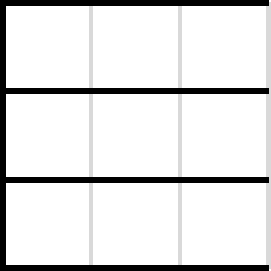
\includegraphics{image/trees-forests/Kruskal-example}
\caption{Kruskal's algorithm for the $4 \times 4$ grid graph.}
\label{fig:trees-forests:Kruskal_example}
\end{figure}


%%%%%%%%%%%%%%%%%%%%%%%%%%%%%%%%%%%%%%%%%%%%%%%%%%%%%%%%%%%%%%%%%%%%%%%%%%%

\subsection{Prim's algorithm}
\label{subsec:trees_forests:Prim_algorithm}
\index{Prim!algorithm}

Like Kruskal's\index{Kruskal!algorithm} algorithm,
Prim's\index{Prim!algorithm} algorithm uses a
greedy\index{algorithm!greedy} approach to computing a
minimum\index{spanning tree!minimum} spanning tree of a connected
weighted\index{graph!weighted} graph $G = (V,E)$, where $n = |V|$ and
$m = |E|$. The algorithm was developed in 1930 by Czech mathematician
V.~Jarn\'ik\index{Jarn\'ik, V.}~\cite{Jarnik1930} and later
independently by R.~C.~Prim\index{Prim!R. C.}~\cite{Prim1957} and
E.~W.~Dijkstra\index{Dijkstra!E. W.}~\cite{Dijkstra1959}. However,
Prim\index{Prim!R. C.} was the first to present an implementation
that runs in time $O(n^2)$. Using $2$-heaps\index{heap!$2$-heap}, the
runtime can be reduced~\cite{KershenbaumVanSlyke1972} to
$O(m \log n)$. With a Fibonacci\index{heap!Fibonacci} heap
implementation~\cite{FredmanTarjan1984,FredmanTarjan1987}, the runtime
can be reduced even further to $O(m + n \log n)$.

Pseudocode of Prim's\index{Prim!algorithm} algorithm is given in
Algorithm~\ref{alg:trees_forests:prim}. For each $v \in V$, $\cost[v]$
denotes the minimum\index{weight!minimum} weight among all edges
connecting $v$ to a vertex in the tree $T$, and $\parent[v]$ denotes
the parent of $v$ in $T$. During the algorithm's execution, vertices
$v$ that are not in $T$ are organized in the
minimum-priority\index{queue!minimum-priority} queue $Q$, prioritized
according to $\cost[v]$. Lines~\ref{alg:prim:for_start:init}
to~\ref{alg:prim:for_end:init} set each $\cost[v]$ to a number that
is larger than any weight in the graph $G$, usually written $\infty$.
The parent of each vertex is set to \texttt{NULL} because we have not
yet started constructing the MST $T$. In
lines~\ref{alg:prim:arbitrary_root}
to~\ref{alg:prim:init_min_priority_queue}, we choose an arbitrary
vertex $r$ from $V$ and mark that vertex as the root of $T$. The
minimum-priority\index{queue!minimum-priority} queue is set to be all
vertices from $V$. We set $\cost[r]$ to zero, making $r$ the only
vertex so far with a cost that is $< \infty$. During the first
execution of the while loop from
lines~\ref{alg:prim:while_start:build_tree}
to~\ref{alg:prim:while_end:build_tree}, $r$ is the first vertex to be
extracted from $Q$ and processed. Line~\ref{alg:prim:extract_min}
extracts a vertex $u$ from $Q$ based on the key $\cost$, thus moving
$u$ to the vertex set of $T$. Line~\ref{alg:prim:neighbors_u}
considers all vertices adjacent to $u$. In an undirected graph, these
are the neighbors of $u$; in a digraph, we replace $\adj(u)$ with the
out-neighbors $\oadj(u)$. The while loop updates the $\cost$ and
$\parent$ fields of each vertex $v$ adjacent to $u$ that is not in
$T$. If $\parent[v] \neq \texttt{NULL}$, then $\cost[v] < \infty$ and
$\cost[v]$ is the weight of an edge connecting $v$ to some vertex
already in $T$. Lines~\ref{alg:prim:MST_edge_set}
to~\ref{alg:prim:return_MST} construct the edge set of the minimum
spanning tree and return this edge set. The proof of correctness of
Algorithm~\ref{alg:trees_forests:prim} is similar to the proof of
Theorem~\ref{thm:trees_forests:correctness_Kruskal_algorithm}.
Figure~\ref{fig:tree_forests:Prim_algorithm_digraph} shows the minimum
spanning tree rooted at vertex $1$ as a result of running Prim's
algorithm over a digraph;
Figure~\ref{fig:tree_forests:Prim_algorithm_undirected_graph} shows
the corresponding tree rooted at vertex $5$ of an undirected graph.

\begin{algorithm}[!htbp]
\index{Prim!algorithm}
\index{spanning tree!minimum}
%%%%%%%%%%%%%%%%%%%%%%%%%%%%%%%%%%%%%%%%%%%%%%%%%%%%%%%%%%%%%%%%%%%%%%%%%%%
%% This file is part of the book
%%
%% Algorithmic Graph Theory
%% http://code.google.com/p/graph-theory-algorithms-book/
%%
%% Copyright (C) 2009, 2010 Minh Van Nguyen <nguyenminh2@gmail.com>
%%
%% See the file COPYING for copying conditions.
%%%%%%%%%%%%%%%%%%%%%%%%%%%%%%%%%%%%%%%%%%%%%%%%%%%%%%%%%%%%%%%%%%%%%%%%%%%

\dontprintsemicolon
%%
%% data section
\SetKwInOut{Input}{Input}
\SetKwInOut{Output}{Output}
%%
%% input/output
\Input{A connected graph $G = (V, E)$ having edge weights.}
\Output{A MST $T$ for $G$.}
\BlankLine
%%
%% algorithm body
Initialize: $V(T) = \{v_0\}$, where $v_0$ is an arbitrary vertex, $E(T)=\emptyset$\;
While $V(T)\not= V$:\;
{
\quad Choose edge $(u,v)$ with minimal weight such that $u$ is in $V(T)$
but $v$ is not,\;
\quad Add $v$ to $V(T)$, add $(u, v)$ to $E(T)$.\;
}

\caption{Prim's algorithm.}
\label{alg:trees_forests:prim}
\end{algorithm}

\begin{lstlisting}
def prim(G):
    """
    Implements Prim's algorithm to compute a MST of a graph.

    INPUT:
        G - a connected graph.
    OUTPUT:
        T - a minimum weight spanning tree.

    REFERENCES:
        http://en.wikipedia.org/wiki/Prim's_algorithm
    """
    T_vertices = [0] # assumes G.vertices = range(n)
    T_edges = []
    E = G.edges() # a list of triples
    V = G.vertices()
    # start ugly hack to sort E
    Er = [list(x) for x in E]
    E0 = []
    for x in Er:
        x.reverse()
        E0.append(x)
    E0.sort()
    E = []
    for x in E0:
        x.reverse()
        E.append(tuple(x))
    # end ugly hack to get E is sorted by weight
    for x in E:
        u = x[0]
        v = x[1]
        if u in T_vertices and not(v in T_vertices):
            T_edges.append([u,v])
            T_vertices.append(v)
    # found T_vertices, T_edges
    # find adj mat of T
    if G.weighted():
        AG = G.weighted_adjacency_matrix()
    else:
        AG = G.adjacency_matrix()
    GV = G.vertices()
    n = len(GV)
    AT = []
    for i in GV:
        rw = [0]*n
        for j in GV:
            if [i,j] in T_edges:
                rw[j] = AG[i][j]
        AT.append(rw)
    AT = matrix(AT)
    return Graph(AT, format = "adjacency_matrix", weighted = True)
\end{lstlisting}

\begin{lstlisting}
sage: A = matrix([[0,1,2,3], [3,0,2,1], [2,1,0,3], [1,1,1,0]])
sage: G = DiGraph(A, format="adjacency_matrix", weighted=True)
sage: E = G.edges(); E
[(0, 1, 1), (0, 2, 2), (0, 3, 3), (1, 0, 3), (1, 2, 2), (1, 3, 1), (2, 0, 2),
(2, 1, 1), (2, 3, 3), (3, 0, 1), (3, 1, 1), (3, 2, 1)]
sage: prim(G)
Multi-graph on 4 vertices
sage: prim(G).edges()
[(0, 1, 1), (0, 2, 2), (1, 3, 1)]
\end{lstlisting}

\begin{figure}[!htbp]
\centering
\index{Prim!algorithm}
\index{spanning tree!minimum}
\subfigure[Original digraph.]{
  \includegraphics{image/trees-forests/Prim-algorithm-digraph_original}
}
\qquad
\subfigure[1st iteration of while loop.]{
  \includegraphics{image/trees-forests/Prim-algorithm-digraph_first}
}
\subfigure[2nd iteration of while loop.]{
  \includegraphics{image/trees-forests/Prim-algorithm-digraph_second}
}
\qquad
\subfigure[Final MST.]{
  \includegraphics{image/trees-forests/Prim-algorithm-digraph_final}
}
\caption{Running Prim's algorithm over a digraph.}
\label{fig:tree_forests:Prim_algorithm_digraph}
\end{figure}

\begin{lstlisting}
sage: A = matrix([[0,7,0,5,0,0,0], [0,0,8,9,7,0,0], [0,0,0,0,5,0,0], \
...  [0,0,0,0,15,6,0], [0,0,0,0,0,8,9], [0,0,0,0,0,0,11], [0,0,0,0,0,0,0]])
sage: G = Graph(A, format="adjacency_matrix", weighted=True)
sage: E = G.edges(); E
[(0, 1, 7), (0, 3, 5), (1, 2, 8), (1, 3, 9), (1, 4, 7), (2, 4, 5),
(3, 4, 15), (3, 5, 6), (4, 5, 8), (4, 6, 9), (5, 6, 11)]
sage: prim(G).edges()
[(0, 1, 7), (0, 3, 5), (1, 2, 8), (1, 4, 7), (3, 5, 6), (4, 6, 9)]
\end{lstlisting}

\begin{figure}[!htbp]
\centering
\index{Prim!algorithm}
\index{spanning tree!minimum}
\subfigure[Original undirected graph.]{
  \includegraphics{image/trees-forests/Prim-algorithm-undirected-graph_original}
}
\qquad
\subfigure[1st iteration of while loop.]{
  \includegraphics{image/trees-forests/Prim-algorithm-undirected-graph_first}
}
\subfigure[2nd iteration of while loop.]{
  \includegraphics{image/trees-forests/Prim-algorithm-undirected-graph_second}
}
\qquad
\subfigure[3rd iteration of while loop.]{
  \includegraphics{image/trees-forests/Prim-algorithm-undirected-graph_third}
}
\subfigure[4th iteration of while loop.]{
  \includegraphics{image/trees-forests/Prim-algorithm-undirected-graph_fourth}
}
\qquad
\subfigure[Final MST.]{
  \includegraphics{image/trees-forests/Prim-algorithm-undirected-graph_final}
}
\caption{Running Prim's algorithm over an undirected graph.}
\label{fig:tree_forests:Prim_algorithm_undirected_graph}
\end{figure}


%%%%%%%%%%%%%%%%%%%%%%%%%%%%%%%%%%%%%%%%%%%%%%%%%%%%%%%%%%%%%%%%%%%%%%%%%%%

\subsection{Bor\r{u}vka's algorithm}
\label{subsec:trees_forests:Boruvka_algorithm}
\index{Bor\r{u}vka!algorithm}

Bor\r{u}vka's
algorithm~\cite{Boruvka1926a,Boruvka1926b}\index{Bor\r{u}vka!algorithm}
is a procedure for finding a minimum\index{spanning tree!minimum}
spanning tree in a weighted connected graph $G = (V,E)$ for which all
edge weights are distinct. It was first published in~1926 by Otakar
Bor\r{u}vka\index{Bor\r{u}vka!Otakar} but subsequently rediscovered
by many others, including
Choquet\index{Choquet, G.}~\cite{Choquet1938} and
Florek\index{Florek, K.}\index{{\L}ukaszewicz, J.}\index{Perkal, J.}\index{Steinhaus, H.}\index{Zubrzycki, S.}~et~al.~\cite{FlorekEtAl1951}.
If $G$ has order $n = |V|$ and size $m = |E|$, it can be shown that
Bor\r{u}vka's\index{Bor\r{u}vka!algorithm} algorithm runs in time
$O(m \log n)$.

\begin{algorithm}[!htbp]
\index{Bor\r{u}vka!algorithm}
\index{spanning tree!minimum}
%%%%%%%%%%%%%%%%%%%%%%%%%%%%%%%%%%%%%%%%%%%%%%%%%%%%%%%%%%%%%%%%%%%%%%%%%%%
%% This file is part of the book
%%
%% Algorithmic Graph Theory
%% http://code.google.com/p/graph-theory-algorithms-book/
%%
%% Copyright (C) 2009, 2010 Minh Van Nguyen <nguyenminh2@gmail.com>
%%
%% See the file COPYING for copying conditions.
%%%%%%%%%%%%%%%%%%%%%%%%%%%%%%%%%%%%%%%%%%%%%%%%%%%%%%%%%%%%%%%%%%%%%%%%%%%

\dontprintsemicolon
%%
%% data section
\SetKwInOut{Input}{Input}
\SetKwInOut{Output}{Output}
\SetKwData{NULL}{NULL}
%%
%% input/output
\Input{A weighted connected graph $G = (V, E)$ with weight function
  $w$. All the edge weights of $G$ are distinct.}
\Output{A minimum spanning tree $T$ of $G$.}
\BlankLine
%%
%% algorithm body
$n \assign |V|$\nllabel{alg:Boruvka:get_graph_order}\;
$T \assign \overline{K}_n$\nllabel{alg:Boruvka:spanning_forest}\;
\While{$|E(T)| < n - 1$\nllabel{alg:Boruvka:while_loop_start}}{
  \For{\rm each component $T'$ of $T$}{
    $e' \assign$ edge of minimum weight that leaves $T'$\;
    $E(T) \assign E(T) \cup e'$\nllabel{alg:Boruvka:while_loop_end}\;
  }
}
\Return $T$\;

\caption{Bor\r{u}vka's algorithm.}
\label{alg:trees_forests:Boruvka}
\end{algorithm}

Algorithm~\ref{alg:trees_forests:Boruvka} provides pseudocode of
Bor\r{u}vka's\index{Bor\r{u}vka!algorithm} algorithm. Given a
weighted connected graph $G = (V,E)$ all of whose edge weights are
distinct, the initialization steps in
lines~\ref{alg:Boruvka:get_graph_order}
and~\ref{alg:Boruvka:spanning_forest} construct a
spanning\index{spanning forest} forest $T$ of $G$, i.e. the subgraph
of $G$ containing all of the latter's vertices and no edges. The
initial forest has $n$ components, each being the
trivial\index{graph!trivial} graph $K_1$. The while loop from
lines~\ref{alg:Boruvka:while_loop_start}
to~\ref{alg:Boruvka:while_loop_end} constructs a spanning tree of $G$
via a recursive\index{recursion} procedure similar to
Theorem~\ref{thm:trees_forests:recursive_construction_trees}. For each
component $T'$ of $T$, we consider all the out-going edges of $T'$ and
choose an edge $e'$ that has minimum\index{weight!minimum} weight
among all such edges. This edge is then added to the edge set of
$T$. In this way, two distinct components, each of which is a tree,
are joined together by a bridge\index{bridge}. At the end of the while
loop, our final graph is a minimum\index{spanning tree!minimum}
spanning tree of $G$. Note that the forest-merging steps in the for
loop from lines~\ref{alg:Boruvka:for_loop}
to~\ref{alg:Boruvka:while_loop_end} are amenable to
parallelization\index{parallelization}, hence the alternative name to
Bor\r{u}vka's\index{Bor\r{u}vka!algorithm} algorithm: the parallel
forest-merging method\index{parallel forest-merging}.

\begin{figure}[!htbp]
\centering
\index{Bor\r{u}vka!algorithm}
\index{recursion}
\index{spanning tree!minimum}
\subfigure[Original undirected graph.]{
  \label{fig:Boruvkas_algorithm:original_undirected_graph}
  \includegraphics{image/trees-forests/Boruvkas-algorithm_original}
}
\qquad
\subfigure[0th iteration of while loop.]{
  \includegraphics{image/trees-forests/Boruvkas-algorithm_zeroth}
}
\subfigure[1st iteration of while loop.]{
  \includegraphics{image/trees-forests/Boruvkas-algorithm_first}
}
\qquad
\subfigure[2nd iteration of while loop.]{
  \label{fig:Boruvkas_algorithm:final_minimum_spanning_tree}
  \includegraphics{image/trees-forests/Boruvkas-algorithm_second}
}
\caption{Recursive construction of MST via Bor\r{u}vka's algorithm.}
\label{fig:trees_forests:Boruvka_algorithm}
\end{figure}

\begin{example}
\rm
Figure~\ref{fig:trees_forests:Boruvka_algorithm} illustrates the
gradual construction of a minimum spanning tree for the undirected
graph given in
Figure~\ref{fig:Boruvkas_algorithm:original_undirected_graph}. In this
case, we require two iterations of the while loop in
Bor\r{u}vka's\index{Bor\r{u}vka!algorithm} algorithm in order to
obtain the final minimum\index{spanning tree!minimum} spanning tree in
Figure~\ref{fig:Boruvkas_algorithm:final_minimum_spanning_tree}.\qed
\end{example}

\begin{lstlisting}
def which_index(x,L):
    """
    L is a list of sublists (or tuple of sets or list
    of tuples, etc).

    Returns the index of the first sublist which x belongs
    to, or None if x is not in flatten(L).

    The 0-th element in
    Lx = [L.index(S) for S in L if x in S]
    almost works, but if the list is empty then Lx[0]
    throws an exception.

    EXAMPLES:
        sage: L = [[1,2,3],[4,5],[6,7,8]]
        sage: which_index(3,L)
        0
        sage: which_index(4,L)
        1
        sage: which_index(7,L)
        2
        sage: which_index(9,L)
        sage: which_index(9,L) == None
        True
    """
    for S in L:
        if x in S:
            return L.index(S)
    return None

def boruvka(G):
    """
    Implements Boruvka's algorithm to compute a MST of a graph.

    INPUT:
        G - a connected edge-weighted graph with distinct weights.
    OUTPUT:
        T - a minimum weight spanning tree.

    REFERENCES:
        http://en.wikipedia.org/wiki/Boruvka's_algorithm
    """
    T_vertices = [] # assumes G.vertices = range(n)
    T_edges = []
    T = Graph()
    E = G.edges() # a list of triples
    V = G.vertices()
    # start ugly hack to sort E
    Er = [list(x) for x in E]
    E0 = []
    for x in Er:
        x.reverse()
        E0.append(x)
    E0.sort()
    E = []
    for x in E0:
        x.reverse()
        E.append(tuple(x))
    # end ugly hack to get E is sorted by weight
    for e in E:
        # create about |V|/2 edges of T "cheaply"
        TV = T.vertices()
        if not(e[0] in TV) or not(e[1] in TV):
           T.add_edge(e)
    for e in E:
        # connect the "cheapest" components to get T
        C = T.connected_components_subgraphs()
        VC = [S.vertices() for S in C]
        if not(e in T.edges()) and (which_index(e[0],VC) != which_index(e[1],VC)):
           if T.is_connected():
                break
            T.add_edge(e)
    return T
\end{lstlisting}

Some examples using Sage:
%
\begin{lstlisting}
sage: A = matrix([[0,1,2,3], [4,0,5,6], [7,8,0,9], [10,11,12,0]])
sage: G = DiGraph(A, format="adjacency_matrix", weighted=True)
sage: boruvka(G)
Multi-graph on 4 vertices
sage: boruvka(G).edges()
[(0, 1, 1), (0, 2, 2), (0, 3, 3)]
sage: A = matrix([[0,2,0,5,0,0,0], [0,0,8,9,7,0,0], [0,0,0,0,1,0,0],\
...   [0,0,0,0,15,6,0], [0,0,0,0,0,3,4], [0,0,0,0,0,0,11], [0,0,0,0,0,0,0]])
sage: G = Graph(A, format="adjacency_matrix", weighted=True)
sage: E = G.edges(); E
[(0, 1, 2), (0, 3, 5), (1, 2, 8), (1, 3, 9), (1, 4, 7),
(2, 4, 1), (3, 4, 15), (3, 5, 6), (4, 5, 3), (4,6, 4), (5, 6, 11)]
sage: boruvka(G)
Multi-graph on 7 vertices
sage: boruvka(G).edges()
[(0, 1, 2), (0, 3, 5), (2, 4, 1), (3, 5, 6), (4, 5, 3), (4, 6, 4)]
sage: A = matrix([[0,1,2,5], [0,0,3,6], [0,0,0,4], [0,0,0,0]])
sage: G = Graph(A, format="adjacency_matrix", weighted=True)
sage: boruvka(G).edges()
[(0, 1, 1), (0, 2, 2), (2, 3, 4)]
sage: A = matrix([[0,1,5,0,4], [0,0,0,0,3], [0,0,0,2,0], [0,0,0,0,0], [0,0,0,0,0]])
sage: G = Graph(A, format="adjacency_matrix", weighted=True)
sage: boruvka(G).edges()
[(0, 1, 1), (0, 2, 5), (1, 4, 3), (2, 3, 2)]
\end{lstlisting}


%%%%%%%%%%%%%%%%%%%%%%%%%%%%%%%%%%%%%%%%%%%%%%%%%%%%%%%%%%%%%%%%%%%%%%%%%%%

\section{Binary trees}
\label{sec:trees_forests:binary_trees}
\index{binary tree}

A \emph{binary tree}\index{binary tree} is a rooted\index{tree!rooted}
tree with at most two children per parent. Each child is designated as
either a \emph{left-child}\index{child!left} or a
\emph{right-child}\index{child!right}. Thus binary\index{binary tree}
trees are also $2$-ary\index{tree!$2$-ary} trees. Some
examples of binary trees are illustrated in
Figure~\ref{fig:trees_forests:examples_binary_trees}. Given a vertex
$v$ in a binary tree $T$ of height $h$, the
\emph{left subtree}\index{subtree!left} of $v$ is comprised of the
subtree that spans the left-child\index{child!left} of $v$ and all
of this child's descendants. The notion of a
\emph{right-subtree}\index{subtree!right} of a
binary\index{binary tree} tree is similarly defined. Each of the
left\index{subtree!left} and right\index{subtree!right} subtrees of
$v$ is itself a binary tree with height $\leq h - 1$. If $v$ is the
root vertex, then each of its left\index{subtree!left} and
right\index{subtree!right} subtrees has height $\leq h - 1$, and at
least one of these subtrees has height equal to $h - 1$.

\begin{figure}[!htbp]
\centering
\index{binary tree}
\subfigure[]{
  \includegraphics{image/trees-forests/example-binary-trees_a}
}
\qquad
\subfigure[]{
  \includegraphics{image/trees-forests/example-binary-trees_b}
}
\qquad
\subfigure[]{
  
\includegraphics{image/trees-forests/example-binary-trees_c}
}
\qquad
\subfigure[]{
  
\includegraphics{image/trees-forests/example-binary-trees_d}
}
\caption{Examples of binary trees.}
\label{fig:trees_forests:examples_binary_trees}
\end{figure}

\begin{theorem}
\label{thm:trees_forests:complete_binary_tree_exact_order}
If $T$ is a complete\index{binary tree!complete} binary tree of height
$h$, then $T$ has $2^{h+1} - 1$ vertices.
\end{theorem}

\begin{proof}
Argue by induction\index{induction} on $h$. The assertion of the
theorem is trivially true in the base case $h = 0$. Let $k \geq 0$ and
assume for induction that any complete binary tree of height $k$ has
order $2^{k+1} - 1$. Suppose $T$ is a
complete\index{binary tree!complete} binary tree of height $k + 1$ and
denote the left\index{subtree!left} and right\index{subtree!right}
subtrees of $T$ by $T_1$ and $T_2$, respectively. Each $T_i$~(for
$i = 1,2$) is a complete\index{binary tree!complete} binary tree of
height $k$ and by our induction hypothesis $T_i$ has $2^{k+1} - 1$
vertices. Thus $T$ has order
\[
1 + (2^{k+1} - 1) + (2^{k+1} - 1)
=
2^{k+2} - 1
\]
as required.
\end{proof}

Theorem~\ref{thm:trees_forests:complete_binary_tree_exact_order}
provides a useful upper bound on the order of a
binary\index{binary tree} tree of a given height. This upper bound is
stated in the following corollary.

\begin{corollary}
A binary tree of height $h$ has at most $2^{h+1} - 1$ vertices.
\end{corollary}

We now count the number of possible binary trees on $n$
vertices. Let $b_n$ be the number of binary trees of order $n$. For
$n = 0$, we set $b_0 = 1$. The trivial graph is the only binary tree
with one vertex, hence $b_1 = 1$. Suppose $n > 1$ and let $T$ be a
binary tree on $n$ vertices. Then the left subtree of $T$ has order
$0 \leq i \leq n - 1$ and the right subtree has $n - 1 - i$
vertices. As there are $b_i$ possible left subtrees and $b_{n-1-i}$
possible right subtrees, $T$ has a total of $b_i b_{n-1-i}$ different
combinations of left and right subtrees. Summing from $i = 0$ to
$i = n - 1$ and we have
%%
\begin{equation}
\label{eqn:trees_forests:Catalan_recursion}
b_n
=
\sum_{i=0}^{n-1} b_i b_{n-1-i}.
\end{equation}
%%
Expression~\eqref{eqn:trees_forests:Catalan_recursion} is known as the
\emph{Catalan recursion}\index{Catalan!recursion} and the number $b_n$
is the $n$-th Catalan\index{Catalan!number} number, which we know from
problem~\ref{chap:introduction}.\ref{prob:introduction:Euler_polygon_division}
can be expressed in the closed\index{closed form} form
%%
\begin{equation}
\label{eqn:trees_forests:nth_Catalan_number_closed_form}
b_n
=
\frac{1}{n+1} \binom{2n}{n}.
\end{equation}
%%
Figures~\ref{fig:trees_forests:binary_trees_2_vertices}
to~\ref{fig:trees_forests:binary_trees_4_vertices} enumerate all the
different binary trees on $2$, $3$, and $4$ vertices, respectively.

\begin{figure}[!htbp]
\centering
\index{binary tree}
%%%%%%%%%%%%%%%%%%%%%%%%%%%%%%%%%%%%%%%%%%%%%%%%%%%%%%%%%%%%%%%%%%%%%%%%%%%
%% This file is part of the book
%%
%% Algorithmic Graph Theory
%% http://code.google.com/p/graph-theory-algorithms-book/
%%
%% Copyright (C) 2009--2011 Minh Van Nguyen <nguyenminh2@gmail.com>
%%
%% See the file COPYING for copying conditions.
%%%%%%%%%%%%%%%%%%%%%%%%%%%%%%%%%%%%%%%%%%%%%%%%%%%%%%%%%%%%%%%%%%%%%%%%%%%

\documentclass{article}

\usepackage{subfigure}
\usepackage{tikz}
\usetikzlibrary{external}
\usetikzlibrary{trees}
\tikzexternalize{binary-trees-2-vertices}

\begin{document}

\begin{figure}
\subfigure[]{
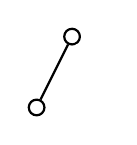
\begin{tikzpicture}
[-,thick,%
  every node/.style={shape=circle,inner sep=2pt,draw,thick},%
  scale=0.6]
\node {}
  child {node {}}
  child[white] {};
\end{tikzpicture}
}
%%
%%
\qquad
\subfigure[]{
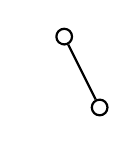
\begin{tikzpicture}
[-,thick,%
  every node/.style={shape=circle,inner sep=2pt,draw,thick},%
  scale=0.6]
\node {}
  child[white] {}
  child {node {}};
\end{tikzpicture}
}
\end{figure}

\end{document}

\caption{The $b_2 = 2$ binary trees on $2$ vertices.}
\label{fig:trees_forests:binary_trees_2_vertices}
\end{figure}

\begin{figure}[!htbp]
\centering
\index{binary tree}
%%%%%%%%%%%%%%%%%%%%%%%%%%%%%%%%%%%%%%%%%%%%%%%%%%%%%%%%%%%%%%%%%%%%%%%%%%%
%% This file is part of the book
%%
%% Algorithmic Graph Theory
%% http://code.google.com/p/graph-theory-algorithms-book/
%%
%% Copyright (C) 2009, 2010, 2011 Minh Van Nguyen <nguyenminh2@gmail.com>
%%
%% See the file COPYING for copying conditions.
%%%%%%%%%%%%%%%%%%%%%%%%%%%%%%%%%%%%%%%%%%%%%%%%%%%%%%%%%%%%%%%%%%%%%%%%%%%

\documentclass{article}

\usepackage{subfigure}
\usepackage{tikz}
\usetikzlibrary{external}
\usetikzlibrary{trees}
\tikzexternalize{binary-trees-3-vertices}

\begin{document}

\begin{figure}
\subfigure[]{
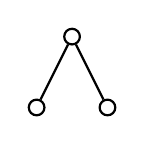
\begin{tikzpicture}
[-,thick,%
  every node/.style={shape=circle,inner sep=2pt,draw,thick},%
  scale=0.6]
\node {}
  child {node {}}
  child {node {}};
\end{tikzpicture}
}
%%
%%
\qquad
\subfigure[]{
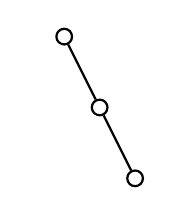
\begin{tikzpicture}
[-,thick,%
  every node/.style={shape=circle,inner sep=2pt,draw,thick},%
  scale=0.6]
\node {}
  child[white] {}
  child {node {}
    child[white] {}
    child {node {}}};
\end{tikzpicture}
}
%%
%%
\qquad
\subfigure[]{
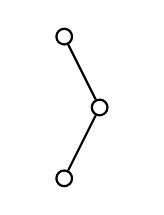
\begin{tikzpicture}
[-,thick,%
  every node/.style={shape=circle,inner sep=2pt,draw,thick},%
  scale=0.6]
\node {}
  child[white] {}
  child {node {}
    child {node {}}
    child[white] {}};
\end{tikzpicture}
}
%%
%%
\qquad
\subfigure[]{
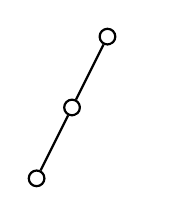
\begin{tikzpicture}
[-,thick,%
  every node/.style={shape=circle,inner sep=2pt,draw,thick},%
  scale=0.6]
\node {}
  child {node {}
    child {node {}}
    child[white] {}}
  child[white] {};
\end{tikzpicture}
}
%%
%%
\qquad
\subfigure[]{
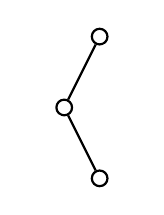
\begin{tikzpicture}
[-,thick,%
  every node/.style={shape=circle,inner sep=2pt,draw,thick},%
  scale=0.6]
\node {}
  child {node {}
    child[white] {}
    child {node {}}}
  child[white] {};
\end{tikzpicture}
}
\end{figure}

\end{document}

\caption{The $b_3 = 5$ binary trees on $3$ vertices.}
\label{fig:trees_forests:binary_trees_3_vertices}
\end{figure}

\begin{figure}[!htbp]
\centering
\index{binary tree}
%%%%%%%%%%%%%%%%%%%%%%%%%%%%%%%%%%%%%%%%%%%%%%%%%%%%%%%%%%%%%%%%%%%%%%%%%%%
%% This file is part of the book
%%
%% Algorithmic Graph Theory
%% http://code.google.com/p/graph-theory-algorithms-book/
%%
%% Copyright (C) 2009, 2010, 2011 Minh Van Nguyen <nguyenminh2@gmail.com>
%%
%% See the file COPYING for copying conditions.
%%%%%%%%%%%%%%%%%%%%%%%%%%%%%%%%%%%%%%%%%%%%%%%%%%%%%%%%%%%%%%%%%%%%%%%%%%%

%% top row
%%
\subfigure[]{
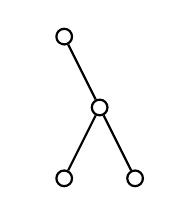
\begin{tikzpicture}
[-,thick,%
  every node/.style={shape=circle,inner sep=2pt,draw,thick},%
  scale=0.6]
\node {}
  child[white] {}
  child {node {}
    child {node {}}
    child {node {}}
  };
\end{tikzpicture}
}
%%
%%
\qquad
\subfigure[]{
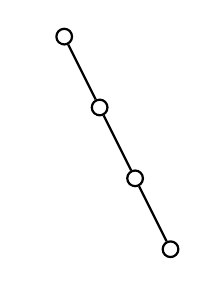
\begin{tikzpicture}
[-,thick,%
  every node/.style={shape=circle,inner sep=2pt,draw,thick},%
  scale=0.6]
\node {}
  child[white] {}
  child {node {}
    child[white] {}
    child {node {}
      child[white] {}
      child {node {}}
    }
  };
\end{tikzpicture}
}
%%
%%
\qquad
\subfigure[]{
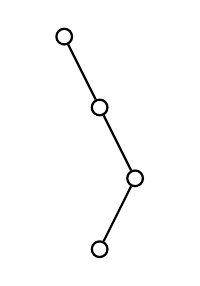
\begin{tikzpicture}
[-,thick,%
  every node/.style={shape=circle,inner sep=2pt,draw,thick},%
  scale=0.6]
\node {}
  child[white] {}
  child {node {}
    child[white] {}
    child {node {}
      child {node {}}
      child[white] {}
    }
  };
\end{tikzpicture}
}
%%
%%
\qquad
\subfigure[]{
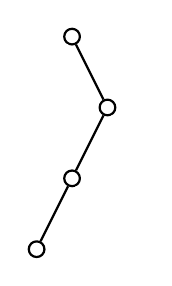
\begin{tikzpicture}
[-,thick,%
  every node/.style={shape=circle,inner sep=2pt,draw,thick},%
  scale=0.6]
\node {}
  child[white] {}
  child {node {}
    child {node {}
      child {node {}}
      child[white] {}
    }
    child[white] {}
  };
\end{tikzpicture}
}
%%
%%
\qquad
\subfigure[]{
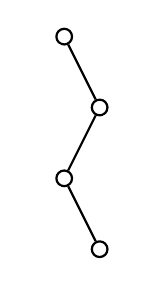
\begin{tikzpicture}
[-,thick,%
  every node/.style={shape=circle,inner sep=2pt,draw,thick},%
  scale=0.6]
\node {}
  child[white] {}
  child {node {}
    child {node {}
      child[white] {}
      child {node {}}
    }
    child[white] {}
  };
\end{tikzpicture}
}
%%
%%
%% middle row
%%
\qquad
\subfigure[]{
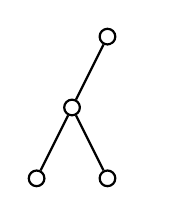
\begin{tikzpicture}
[-,thick,%
  every node/.style={shape=circle,inner sep=2pt,draw,thick},%
  scale=0.6]
\node {}
  child {node {}
    child {node {}}
    child {node {}}
  }
  child[white] {};
\end{tikzpicture}
}
%%
%%
\qquad
\subfigure[]{
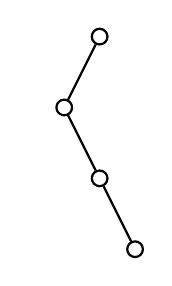
\begin{tikzpicture}
[-,thick,%
  every node/.style={shape=circle,inner sep=2pt,draw,thick},%
  scale=0.6]
\node {}
  child {node {}
    child[white] {}
    child {node {}
      child[white] {}
      child {node {}}
    }
  }
  child[white] {};
\end{tikzpicture}
}
%%
%%
\qquad
\subfigure[]{
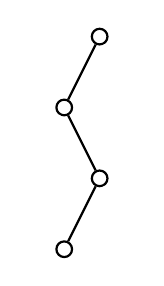
\begin{tikzpicture}
[-,thick,%
  every node/.style={shape=circle,inner sep=2pt,draw,thick},%
  scale=0.6]
\node {}
  child {node {}
    child[white] {}
    child {node {}
      child {node {}}
      child[white] {}
    }
  }
  child[white] {};
\end{tikzpicture}
}
%%
%%
\qquad
\subfigure[]{
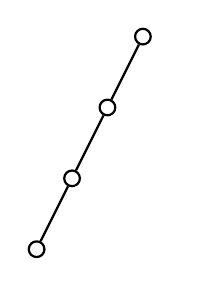
\begin{tikzpicture}
[-,thick,%
  every node/.style={shape=circle,inner sep=2pt,draw,thick},%
  scale=0.6]
\node {}
  child {node {}
    child {node {}
      child {node {}}
      child[white] {}
    }
    child[white] {}
  }
  child[white] {};
\end{tikzpicture}
}
%%
%%
\qquad
\subfigure[]{
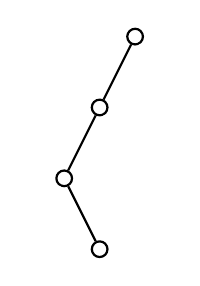
\begin{tikzpicture}
[-,thick,%
  every node/.style={shape=circle,inner sep=2pt,draw,thick},%
  scale=0.6]
\node {}
  child {node {}
    child {node {}
      child[white] {}
      child {node {}}
    }
    child[white] {}
  }
  child[white] {};
\end{tikzpicture}
}
%%
%%
%% last row
%%
\qquad
\subfigure[]{
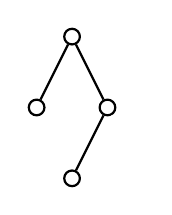
\begin{tikzpicture}
[-,thick,%
  every node/.style={shape=circle,inner sep=2pt,draw,thick},%
  scale=0.6]
\node {}
  child {node {}}
  child {node {}
    child {node {}}
    child[white] {}
  };
\end{tikzpicture}
}
%%
%%
\qquad
\subfigure[]{
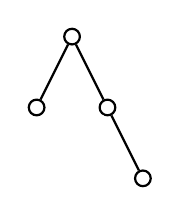
\begin{tikzpicture}
[-,thick,%
  every node/.style={shape=circle,inner sep=2pt,draw,thick},%
  scale=0.6]
\node {}
  child {node {}}
  child {node {}
    child[white] {}
    child {node {}}
  };
\end{tikzpicture}
}
%%
%%
\qquad
\subfigure[]{
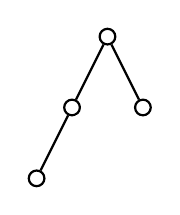
\begin{tikzpicture}
[-,thick,%
  every node/.style={shape=circle,inner sep=2pt,draw,thick},%
  scale=0.6]
\node {}
  child {node {}
    child {node {}}
    child[white] {}
  }
  child {node {}};
\end{tikzpicture}
}
%%
%%
\qquad
\subfigure[]{
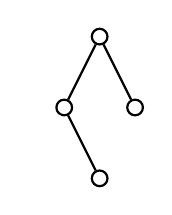
\begin{tikzpicture}
[-,thick,%
  every node/.style={shape=circle,inner sep=2pt,draw,thick},%
  scale=0.6]
\node {}
  child {node {}
    child[white] {}
    child {node {}}
  }
  child {node {}};
\end{tikzpicture}
}

\caption{The $b_4 = 14$ binary trees on $4$ vertices.}
\label{fig:trees_forests:binary_trees_4_vertices}
\end{figure}

The first few values
of~\eqref{eqn:trees_forests:nth_Catalan_number_closed_form} are
\[
b_0 = 1,\quad
b_1 = 1,\quad
b_2 = 2,\quad
b_3 = 5,\quad
b_4 = 14
\]
which are rather small and of manageable size if we want to explicitly
enumerate all different binary trees with the above orders. However,
from $n = 4$ onwards the value of $b_n$ increases very fast. Instead
of enumerating all the $b_n$ different binary trees of a specified
order $n$, a related problem is generating a random binary tree of
order $n$. That is, we consider the set $B$ as a
sample\index{probability!sample space} space of $b_n$ different binary
trees on $n$ vertices, and choose a random\index{element!random}
element from $B$. Such a random\index{element!random} element can be
generated using
Algorithm~\ref{alg:trees_forests:random_binary_tree}. The list
\texttt{parent} holds all vertices with less than two children, each
vertex can be considered as a candidate parent to which we can add a
child. An element of \texttt{parent} is a two-tuple $(v, k)$ where the
vertex $v$ currently has $k$ children.

\begin{algorithm}[!htbp]
\index{binary tree!random}
%%%%%%%%%%%%%%%%%%%%%%%%%%%%%%%%%%%%%%%%%%%%%%%%%%%%%%%%%%%%%%%%%%%%%%%%%%%
%% This file is part of the book
%%
%% Algorithmic Graph Theory
%% http://code.google.com/p/graph-theory-algorithms-book/
%%
%% Copyright (C) 2009--2011 Minh Van Nguyen <nguyenminh2@gmail.com>
%%
%% See the file COPYING for copying conditions.
%%%%%%%%%%%%%%%%%%%%%%%%%%%%%%%%%%%%%%%%%%%%%%%%%%%%%%%%%%%%%%%%%%%%%%%%%%%

\DontPrintSemicolon
\SetAlgoNoLine
%%
%% data section
\SetKwData{Parent}{parent}
%%
%% input
\KwIn{Positive integer $n$.}
%%
%% output
\KwOut{A random binary tree on $n$ vertices.}
\BlankLine
%%
%% algorithm body
\If{$n = 1$}{
  \Return $K_1$\;
}
$v \assign 0$\;
$T \assign$ null graph\;
add $v$ to $T$\;
$\Parent \assign [(v,0)]$\;
\For{$i \assign 1, 2, \dots, n-1$}{
  $(v,k) \assign$ remove random element from \Parent\;
  \If{$k < 1$}{
    add $(v, k+1)$ to \Parent\;
  }
  add edge $(v, i)$ to $T$\;
  add $(i, 0)$ to \Parent\;
}
\Return $T$\;

\caption{Random binary tree.}
\label{alg:trees_forests:random_binary_tree}
\end{algorithm}


%%%%%%%%%%%%%%%%%%%%%%%%%%%%%%%%%%%%%%%%%%%%%%%%%%%%%%%%%%%%%%%%%%%%%%%%%%%

\subsection{Binary codes}
\index{code!binary}


%%%%%%%%%%%%%%%%%%%%%%%%%%%%%%%%%%%%%%%%%%%%%%%%%%%%%%%%%%%%%%%%%%%%%%%%%%%

\subsubsection{What is a code?}

A \emph{code}\index{code} is a rule for converting data in one format,
or well-defined tangible representation, into sequences of symbols in
another format. The finite set of symbols used is called the
\emph{alphabet}\index{alphabet}. We shall identify a code as a finite
set of symbols which are the image of the alphabet under this
conversion rule. The elements of this set are referred to as
\emph{codewords}\index{codeword}. For example, using the
ASCII\index{ASCII} code, the letters in the
English\index{alphabet!English} alphabet get converted into numbers in
the set $\{0, 1, \dots, 255\}$. If these numbers are written in
binary, then each codeword\index{codeword} of a letter has length $8$,
i.e. eight bits. In this way, we can reformat or encode a
``string''\index{string} into a sequence of binary\index{bit}
symbols, i.e. $0$'s and $1$'s. \emph{Encoding}\index{encode} is
the conversion process one way. \emph{Decoding}\index{decode} is the
reverse process, converting these sequences of code-symbols back into
information in the original format.

Codes are used for:
%%
\begin{itemize}
\item \emph{Economy}\index{code!economy}. Sometimes this is called
  \emph{entropy encoding}\index{entropy!encoding} since there is an
  entropy\index{entropy!function} function which describes how much
  information\index{information channel} a channel~(with a given
  error\index{error rate} rate) can carry and such codes are designed
  to maximize entropy as best as possible. In this case, in addition
  to simply being given an alphabet\index{alphabet} $\cA$, one might
  be given a \emph{weighted alphabet}\index{alphabet!weighted},
  i.e. an alphabet for which each symbol $a \in \cA$ is associated
  with a nonnegative number $w_a \geq 0$~(in practice, this number
  represents the probability that the symbol $a$ occurs in a typical
  word).

\item \emph{Reliability}\index{code!reliability}. Such codes are
  called \emph{error-correcting codes}\index{code!error-correcting},
  since such codes are designed to communicate information over a
  noisy\index{noisy channel} channel in such a way that the errors in
  transmission are likely to be correctable.

\item \emph{Security}\index{code!security}. Such codes are called
  \emph{cryptosystems}\index{cryptosystem}. In this case, the inverse
  of the coding function $c: \cA \to B^*$ is designed to be
  computationally infeasible. In other words, the
  coding\index{coding function} function $c$ is designed to be a
  \emph{trapdoor function}\index{trapdoor function}.
\end{itemize}
%%
Other codes are merely simpler ways to communicate
information~(e.g.~flag\index{flag semaphore} semaphores,
color\index{color code} codes, genetic\index{genetic code} codes,
braille\index{braille} codes, musical\index{musical score} scores,
chess\index{chess} notation, football\index{football} diagrams, and so
on) and have little or no mathematical structure. We shall not study
them.


%%%%%%%%%%%%%%%%%%%%%%%%%%%%%%%%%%%%%%%%%%%%%%%%%%%%%%%%%%%%%%%%%%%%%%%%%%%

\subsubsection{Basic definitions}

If every word in the code has the same length, the code is called a
\emph{block code}\index{code!block}. If a code is not a block code,
then it is called a \emph{variable-length}\index{code!variable-length}
code. A \emph{prefix-free}\index{code!prefix-free} code is a
code~(typically one of variable-length) with the property that there
is no valid codeword in the code that is a prefix or start of any
other codeword.\footnote{
  In other words, a codeword $s = s_1 \cdots s_m$ is a
  \emph{prefix}\index{code!prefix} of a codeword $t = t_1 \cdots t_n$
  if and only if $m \leq n$ and $s_1 = t_1, \dots, s_m = t_m$. Codes
  that are prefix-free\index{code!prefix-free} are easier to decode
  than codes that are not prefix-free.
}
This is the \emph{prefix-free condition}\index{prefix-free condition}.

One example of a prefix-free\index{code!prefix-free} code is the
ASCII\index{ASCII} code. Another example is
\[
00,\, 01,\, 100.
\]
On the other hand, a non-example is the code
\[
00,\, 01,\, 010,\, 100
\]
since the second codeword is a prefix of the third one. Another
non-example is Morse\index{Morse code} code recalled in
Table~\ref{tab:trees_forests:Morse_code}, where we use $0$ for
``$\cdot$'' (``dit'') and $1$ for ``$-$'' (``dah''). For example,
consider the Morse code for \tta and the Morse\index{Morse code} code
for \ttw. These codewords violate the prefix-free condition.

\begin{table}[!htbp]
\centering
\index{Morse code}
%%%%%%%%%%%%%%%%%%%%%%%%%%%%%%%%%%%%%%%%%%%%%%%%%%%%%%%%%%%%%%%%%%%%%%%%%%%
%% This file is part of the book
%%
%% Algorithmic Graph Theory
%% http://code.google.com/p/graph-theory-algorithms-book/
%%
%% Copyright (C) 2009, 2010, 2011 Minh Van Nguyen <nguyenminh2@gmail.com>
%%
%% See the file COPYING for copying conditions.
%%%%%%%%%%%%%%%%%%%%%%%%%%%%%%%%%%%%%%%%%%%%%%%%%%%%%%%%%%%%%%%%%%%%%%%%%%%

\begin{tabular}{cc|cc} \hline
\ttA & 01    & \ttN & 10 \\
\ttB & 1000  & \ttO & 111 \\
\ttC & 1010  & \ttP & 0110 \\
\ttD & 100   & \ttQ & 1101 \\
\ttE & 0     & \ttR & 010 \\
\ttF & 0010  & \ttS & 000 \\
\ttG & 110   & \ttT & 1 \\
\ttH & 0000  & \ttU & 001 \\
\ttI & 00    & \ttV & 0001 \\
\ttJ & 0111  & \ttW & 011 \\
\ttK & 101   & \ttX & 1001 \\
\ttL & 0100  & \ttY & 1011 \\
\ttM & 11    & \ttZ & 1100 \\\hline
\end{tabular}

\caption{Morse code}
\label{tab:trees_forests:Morse_code}
\end{table}


%%%%%%%%%%%%%%%%%%%%%%%%%%%%%%%%%%%%%%%%%%%%%%%%%%%%%%%%%%%%%%%%%%%%%%%%%%%

\subsubsection{Gray codes}
\index{Gray code}

We begin with some history.\footnote{
  This history comes from an unpublished section~7.2.1.1
  (``Generating all $n$-tuples'') in volume~4 of
  Donald Knuth's\index{Knuth!Donald E.}
  \emph{The Art of Computer Programming}.
}
Frank Gray\index{Gray, Frank}~(1887--1969) wrote about the so-called
Gray\index{Gray code} codes in a~1951 paper published in the Bell
System Technical Journal and then in~1953 patented a device~(used for
television sets) based on his paper. However, the idea of a
binary\index{Gray code!binary} Gray code appeared earlier. In fact, it
appeared in an earlier patent~(one by Stibitz in~1943). It
was also used in the French engineer E.~Baudot's\index{Baudot, E.}
telegraph\index{telegraph} machine of~1878 and in a French booklet by
L.~Gros\index{Gros, L.} on the solution published in~1872 to the
Chinese ring\index{Chinese ring puzzle} puzzle.

The term ``Gray code''\index{Gray code} is ambiguous. It is actually a
large family of sequences of $n$-tuples. Let
$\Z_m = \{0, 1, \dots, m-1\}$. More precisely, an
\emph{$m$-ary Gray code of length $n$}\index{Gray code!$m$-ary}~(called
a \emph{binary Gray code}\index{Gray code!binary} when $m = 2$) is a
sequence of all possible~(i.e. $N = m^n$) $n$-tuples
\[
g_1, g_2, \dots, g_N
\]
where
%%
\begin{itemize}
\item each $g_i \in \Z_m^n$,

\item $g_i$ and $g_{i+1}$ differ by $1$ in exactly one coordinate.
\end{itemize}
%%
In other words, an $m$-ary Gray code of length $n$ is a particular way
to order the set of all $m^n$ $n$-tuples whose coordinates are taken
from $\Z_m$. From the transmission/communication perspective, this
sequence has two advantages:
%%
\begin{itemize}
\item It is easy and fast to produce the sequence, since successive
  entries differ in only one coordinate.

\item An error is relatively easy to detect, since we can compare an
  $n$-tuple with the previous one. If they differ in more than one
  coordinate, we conclude that an error was made.
\end{itemize}

\begin{example}
\rm
Here is a $3$-ary Gray code of length $2$:
\[
[0,0],\; [1,0],\; [2,0],\; [2,1],\; [1,1],\; [0,1],\; [0,2],\;
[1,2],\; [2,2]
\]
and the sequence
\[
[0,0,0],\; [1,0,0],\; [1,1,0],\; [0,1,0],\; [0,1,1],\;
[1,1,1],\; [1,0,1],\; [0,0,1]
\]
is a binary Gray code of length $3$. \qed
\end{example}

Gray codes have applications to engineering, recreational
mathematics~(solving the Tower of
Hanoi\index{Tower of Hanoi puzzle} puzzle, The
Brain\index{The Brain puzzle} puzzle, the Chinese
ring\index{Chinese ring puzzle}  puzzle, etc.), and to
mathematics~(e.g. aspects of combinatorics\index{combinatorics},
computational\index{group theory!computational} group theory, and the
computational aspects of linear\index{code!linear} codes).


%%%%%%%%%%%%%%%%%%%%%%%%%%%%%%%%%%%%%%%%%%%%%%%%%%%%%%%%%%%%%%%%%%%%%%%%%%%

\subsubsection{Binary Gray codes}
\index{Gray code!binary}

Consider the so-called $n$-hypercube\index{hypercube graph} graph
$Q_n$, whose first few instances are illustrated in
Figure~\ref{fig:introduction:hypercube_graphs}. This can be envisioned
as the graph whose vertices are the vertices of a cube in
$n$-space\index{$n$-space}
\[
\{(x_1, \dots, x_n) \mid 0 \leq x_i \leq 1\}
\]
and whose edges are those line segments in $\R^n$ connecting two
\emph{neighboring} vertices, i.e. two vertices that differ in exactly
one coordinate. A binary\index{Gray code!binary} Gray code of length
$n$ can be regarded as a
path on the hypercube\index{hypercube graph} graph $Q_n$ that visits
each vertex of the cube exactly once. In other words, a binary Gray
code of length $n$ may be identified with a
Hamiltonian\index{path!Hamiltonian} path on the graph $Q_n$. For
example, Figure~\ref{fig:trees_forests:gray_code_cube} illustrates a
Hamiltonian\index{path!Hamiltonian} path on $Q_3$.

\begin{figure}[!htbp]
\centering
\index{hypercube graph}
\index{path!Hamiltonian}
%%%%%%%%%%%%%%%%%%%%%%%%%%%%%%%%%%%%%%%%%%%%%%%%%%%%%%%%%%%%%%%%%%%%%%%%%%%
%% This file is part of the book
%%
%% Algorithmic Graph Theory
%% http://code.google.com/p/graph-theory-algorithms-book/
%%
%% Copyright (C) 2009, 2010, 2011 Minh Van Nguyen <nguyenminh2@gmail.com>
%%
%% See the file COPYING for copying conditions.
%%%%%%%%%%%%%%%%%%%%%%%%%%%%%%%%%%%%%%%%%%%%%%%%%%%%%%%%%%%%%%%%%%%%%%%%%%%

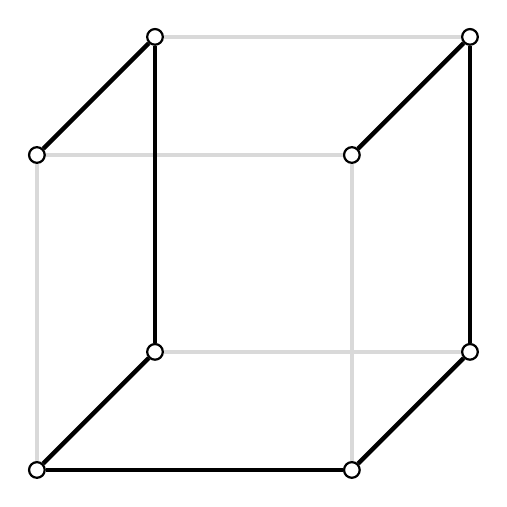
\begin{tikzpicture}
[nodedecorate/.style={shape=circle,inner sep=2pt,draw,thick},%
  darkline/.style={-,ultra thick},
  lightline/.style={-,ultra thick,color=gray!30}]
% nodes or vertices
% foreground square
\node (1) at (0,0) [nodedecorate] {};
\node (2) at (4,0) [nodedecorate] {};
\node (3) at (4,4) [nodedecorate] {};
\node (4) at (0,4) [nodedecorate] {};
% background square
\node (5) at (1.5,1.5) [nodedecorate] {};
\node (6) at (5.5,1.5) [nodedecorate] {};
\node (7) at (5.5,5.5) [nodedecorate] {};
\node (8) at (1.5,5.5) [nodedecorate] {};
% edges or lines
\path
% foreground square
(1) edge[darkline] node {} (2)
(2) edge[lightline] node {} (3)
(3) edge[lightline] node {} (4)
(4) edge[lightline] node {} (1)
% background square
(5) edge[lightline] node {} (6)
(6) edge[darkline] node {} (7)
(7) edge[lightline] node {} (8)
(8) edge[darkline] node {} (5)
% joining foreground and background squares
(1) edge[darkline] node {} (5)
(2) edge[darkline] node {} (6)
(3) edge[darkline] node {} (7)
(4) edge[darkline] node {} (8);
\end{tikzpicture}

\caption{Viewing $\Gamma_3$ as a Hamiltonian path on $Q_3$.}
\label{fig:trees_forests:gray_code_cube}
\end{figure}

How do we efficiently compute a Gray\index{Gray code} code? Perhaps
the simplest way to state the idea of quickly constructing the
\emph{reflected binary Gray code}\index{Gray code!reflected}
$\Gamma_n$ of length $n$ is as follows:
%%
\begin{align*}
\Gamma_0 &= [\,], \\[4pt]
\Gamma_{n} &= \big[[0, \Gamma_{n-1}],\, [1, \Gamma_{n-1}^{\rm rev}]\big]
\end{align*}
%%
where $\Gamma_m^{\rm rev}$ means the Gray code in reverse order. For
instance, we have
%%
\begin{align*}
\Gamma_0 &= [\,], \\[4pt]
\Gamma_1 &= \big[[0],\, [1]\big], \\[4pt]
\Gamma_2 &= \big[[0,0],\, [0,1],\, [1,1],\, [1,0]\big]
\end{align*}
%%
and so on. This is a nice procedure for creating the entire list at
once, which gets very long very fast. An implementation of the
reflected Gray code using Python is given below.

\begin{lstlisting}
def graycode(length,modulus):
    """
    Returns the n-tuple reflected Gray code mod m.


    EXAMPLES:
        sage: graycode(2,4)

        [[0, 0],
         [1, 0],
         [2, 0],
         [3, 0],
         [3, 1],
         [2, 1],
         [1, 1],
         [0, 1],
         [0, 2],
         [1, 2],
         [2, 2],
         [3, 2],
         [3, 3],
         [2, 3],
         [1, 3],
         [0, 3]]
    """
    n,m = length,modulus
    F = range(m)
    if n == 1:
        return [[i] for i in F]
    L = graycode(n-1, m)
    M = []
    for j in F:
        M = M+[ll+[j] for ll in L]
    k = len(M)
    Mr = [0]*m
    for i in range(m-1):
        i1 = i*int(k/m)       # this requires Python 3.0 or Sage
        i2 = (i+1)*int(k/m)
        Mr[i] = M[i1:i2]
    Mr[m-1] = M[(m-1)*int(k/m):]
    for i in range(m):
        if is_odd(i):
            Mr[i].reverse()
    M0 = []
    for i in range(m):
        M0 = M0+Mr[i]
    return M0
\end{lstlisting}

\vskip 0.2in
Consider the reflected\index{Gray code!reflected} binary code of
length $8$, i.e. $\Gamma_8$. This has $2^8 = 256$ codewords. Sage can
easily create the list plot of the coordinates $(x,y)$, where $x$ is
an integer $j \in \Z_{256}$ that indexes the codewords in $\Gamma_8$
and the corresponding $y$ is the $j$-th codeword in $\Gamma_8$
converted to decimal. This will give us some idea of how the Gray code
``looks'' in some sense. The plot is given in
Figure~\ref{fig:trees_forests:Gamma_8}.

\begin{figure}[!htbp]
\centering
\index{Gray code!reflected}
\index{scatterplot}
%%%%%%%%%%%%%%%%%%%%%%%%%%%%%%%%%%%%%%%%%%%%%%%%%%%%%%%%%%%%%%%%%%%%%%%%%%%
%% This file is part of the book
%%
%% Algorithmic Graph Theory
%% http://code.google.com/p/graph-theory-algorithms-book/
%%
%% Copyright (C) 2009--2011 Minh Van Nguyen <nguyenminh2@gmail.com>
%%
%% See the file COPYING for copying conditions.
%%%%%%%%%%%%%%%%%%%%%%%%%%%%%%%%%%%%%%%%%%%%%%%%%%%%%%%%%%%%%%%%%%%%%%%%%%%

\documentclass{article}

\usepackage{pgfplots}
\usepackage{tikz}
\usetikzlibrary{external}
\tikzexternalize{gamma8}

\begin{document}

\begin{figure}
\begin{tikzpicture}
[every mark/.append style={scale=0.3},%
 scale=1]
\begin{axis}
\addplot+[only marks] file {data/trees-forests/gamma8.dat};
\end{axis}
\end{tikzpicture}
\end{figure}

\end{document}

\caption{Scatterplot of $\Gamma_8$.}
\label{fig:trees_forests:Gamma_8}
\end{figure}

What if we only want to compute the $i$-th Gray codeword in the Gray
code of length $n$? Can it be computed quickly without computing the
entire list? At least in the case of the reflected binary Gray code,
there is a very simple way to do this. The $k$-th element in the
above-described reflected binary Gray code of length $n$ is obtained
by simply adding the binary representation of $k$ to the binary
representation of the integer part of $k / 2$. An example using Sage
is given below.

\begin{lstlisting}
def int2binary(m, n):
    '''
    returns GF(2) vector of length n obtained
    from the binary repr of m, padded by 0's
    (on the left) to length n.

    EXAMPLES:
        sage: for j in range(8):
        ....:     print int2binary(j,3)+int2binary(int(j/2),3)
        ....:
        (0, 0, 0)
        (0, 0, 1)
        (0, 1, 1)
        (0, 1, 0)
        (1, 1, 0)
        (1, 1, 1)
        (1, 0, 1)
        (1, 0, 0)
    '''
    s = bin(m)
    k = len(s)
    F = GF(2)
    b = [F(0)]*n
    for i in range(2,k):
        b[n-k+i] = F(int(s[i]))
    return vector(b)

def graycodeword(m, n):
    '''
    returns the k-th codeword in the reflected binary Gray code
    of length n.

    EXAMPLES:
        sage: graycodeword(3,3)
        (0, 1, 0)
    '''
    return map(int, int2binary(m,n)+int2binary(int(m/2),n))
\end{lstlisting}


%%%%%%%%%%%%%%%%%%%%%%%%%%%%%%%%%%%%%%%%%%%%%%%%%%%%%%%%%%%%%%%%%%%%%%%%%%%

\section{Huffman codes}
\label{sec:trees_forests:Huffman_codes}

An \emph{alphabet}\index{alphabet} $\cA$ is a finite set whose
elements are referred to as \emph{symbols}\index{symbol}. A
\emph{word}\index{word}~(or \emph{string}\index{string} or
\emph{message}\index{message}) over $\cA$ is a finite sequence of
symbols in $\cA$ and the \emph{length} of the word is the number of
symbols it contains. A word is usually written by concatenating
symbols together, e.g. $a_1 a_2 \cdots a_k$ ($a_i \in \cA$) is a word
of length $k$.

A commonly occurring alphabet in practice is the
\emph{binary alphabet}\index{alphabet!binary} $\B = \{0, 1\}$. A word
over the binary alphabet is a finite sequence of $0$'s\index{bit} and
$1$'s. If $\cA$ is an alphabet, let $\cA^*$ denote the set of all
words in $\cA$. The length of a word is denoted by vertical bars. That
is, if $w = a_1 \cdots a_k$ is a word over $\cA$, then define
$|w|: \cA^* \to \Z$ by
\[
|w|
=
|a_1 \cdots a_k|
=
k.
\]
Let $\cA$ and $\cB$ be two alphabets. A \emph{code}\index{code} for
$\cA$ using $\cB$ is an injection $c: \cA \to \cB^*$. By abuse of
notation, we often denote the code simply by the set
\[
C
=
c(A)
=
\{c(a) \mid a \in \cA\}.
\]
The elements of $C$ are called \emph{codewords}\index{codeword}. If
$\cB$ is the binary alphabet, then $C$ is called a
\emph{binary code}\index{code!binary}.


%%%%%%%%%%%%%%%%%%%%%%%%%%%%%%%%%%%%%%%%%%%%%%%%%%%%%%%%%%%%%%%%%%%%%%%%%%%

\subsection{Tree representation}
\index{code!tree representation}

Any binary\index{code!binary} code can be represented by a tree, as
Example~\ref{eg:tree_forests:binary_code_tree_representation} shows.

\begin{example}
\label{eg:tree_forests:binary_code_tree_representation}
Let $\B_\ell$ be the binary\index{code!binary} code of length
$\leq \ell$. Represent codewords of $\B_\ell$ using trees.
\end{example}

\begin{proof}[Solution]
Here is how to represent the code $\B_\ell$ consisting of all binary
strings of length $\leq \ell$. Start with the
root\index{vertex!root} node $\varepsilon$\index{$\varepsilon$}
being the empty string. The two children of this node, $v_0$ and
$v_1$, correspond to the two strings of length $1$. Label $v_0$ with a
``$0$'' and $v_1$ with a ``$1$''. The two children of $v_0$,
i.e. $v_{00}$ and $v_{01}$, correspond to the strings of length $2$
which start with a $0$. Similarly, the two children of $v_1$,
i.e. $v_{10}$ and $v_{11}$, correspond to the strings of length $2$
that each starts with a $1$. Continue creating child nodes until we
reach length $\ell$, at which point we stop. There are a total of
$2^{\ell + 1} - 1$ nodes in this tree and $2^\ell$ of them are
leaves\index{vertex!leaf}~(vertices of a tree with degree $1$, i.e. childless
nodes). Note that the parent of any node is a prefix to that
node. Label each node $v_s$ with the string ``$s$'', where $s$ is a
binary sequence of length $\leq \ell$. See
Figure~\ref{fig:trees_forests:tree_representation_B_2} for an example
when $\ell = 2$.
\end{proof}

\begin{figure}[!htbp]
\centering
\index{code!tree representation}
%%%%%%%%%%%%%%%%%%%%%%%%%%%%%%%%%%%%%%%%%%%%%%%%%%%%%%%%%%%%%%%%%%%%%%%%%%%
%% This file is part of the book
%%
%% Algorithmic Graph Theory
%% http://code.google.com/p/graph-theory-algorithms-book/
%%
%% Copyright (C) 2009--2011 Minh Van Nguyen <nguyenminh2@gmail.com>
%%
%% See the file COPYING for copying conditions.
%%%%%%%%%%%%%%%%%%%%%%%%%%%%%%%%%%%%%%%%%%%%%%%%%%%%%%%%%%%%%%%%%%%%%%%%%%%

\documentclass{article}

\usepackage{tikz}
\usetikzlibrary{external}
\tikzexternalize{tree-representation-B-2}

\begin{document}

\begin{figure}
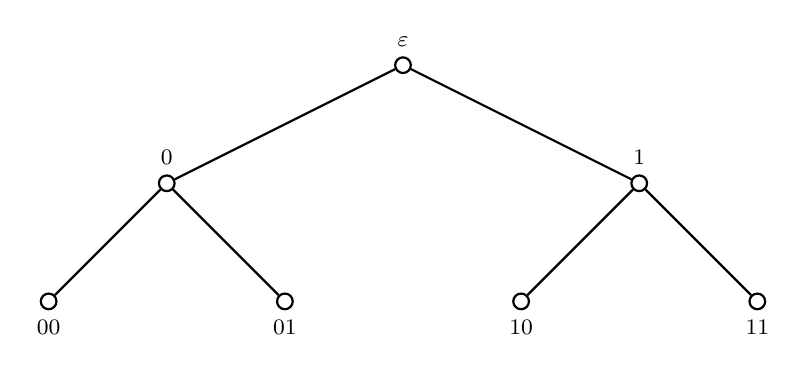
\begin{tikzpicture}
[lineDecorate/.style={-,thick},%
  nodeDecorate/.style={shape=circle,inner sep=2pt,draw,thick},%
  scale=1.5]
%% nodes or vertices
\foreach \nodename/\x/\y/\direction/\navigate in {
  00/0/0/below/south, 01/2/0/below/south, 10/4/0/below/south,
  11/6/0/below/south, 0/1/1/above/north, 1/5/1/above/north}
{
  \node (\nodename) at (\x,\y) [nodeDecorate] {};
  \node [\direction] at (\nodename.\navigate) {\footnotesize$\nodename$};
}
\node (e) at (3,2) [nodeDecorate] {};
\node [above] at (e.north) {\footnotesize$\varepsilon$};
%% edges or lines
\path
\foreach \startnode/\endnode in {0/00, 0/01, 1/10, 1/11, e/0, e/1}
{
  (\startnode) edge[lineDecorate] node {} (\endnode)
};
\end{tikzpicture}
\end{figure}

\end{document}

\caption{Tree representation of the binary code $\B_2$.}
\label{fig:trees_forests:tree_representation_B_2}
\end{figure}

In general, if $C$ is a code contained in $\B_\ell$, then to create
the tree\index{code!tree representation} for $C$, start with the tree
for $\B_\ell$. First, remove all nodes associated to a binary string
for which it and all of its descendants are not in $C$. Next, remove
all labels which do not correspond to codewords in $C$. The resulting
labeled graph is the tree associated to the binary code $C$.

For visualizing the construction of Huffman\index{Huffman code} codes
later, it is important to see that we can \emph{reverse} this
construction to start from such a binary\index{tree!binary} tree and
recover a binary\index{code!binary} code from it. The codewords are
determined by the following rules:
%%
\begin{itemize}
\item The root node gets the empty codeword.

\item Each left-ward branch gets a $0$ appended to the end of its
  parent. Each right-ward branch gets a $1$ appended to the end.
\end{itemize}


%%%%%%%%%%%%%%%%%%%%%%%%%%%%%%%%%%%%%%%%%%%%%%%%%%%%%%%%%%%%%%%%%%%%%%%%%%%

\subsection{Uniquely decodable codes}

If $c: \cA \to \cB^*$ is a code, then we can extend $c$ to $\cA^*$ by
concatenation:
\[
c(a_1 a_2 \cdots a_k)
=
c(a_1) c(a_2) \cdots c(a_k).
\]
If the extension $c: \cA^* \to \cT^*$ is also an injection, then $c$
is called \emph{uniquely decodable}\index{code!uniquely decodable}.
The property of unique decodability or decipherability informally
means that any given sequence of symbols has at most one
interpretation as a sequence of codewords.

\begin{example}
Is the Morse code\index{Morse code} in
Table~\ref{tab:trees_forests:Morse_code} uniquely decodable? Why or
why not?
\end{example}

\begin{proof}[Solution]
Note that these Morse codewords all have lengths less than or equal to
$4$. Other commonly occurring symbols used~(the digits $0$ through
$9$, punctuation symbols, and some others) are also encodable in Morse
code, but they use longer codewords.

Let $\cA$ denote the English alphabet, $\B = \{0, 1\}$ the
binary\index{alphabet!binary} alphabet, and $c: \cA \to \B^*$ the
Morse\index{Morse code} code. Since $c(ET) = 01 = c(A)$, it is clear
that the Morse code is \emph{not} uniquely decodable.
\end{proof}

In fact, prefix-free implies uniquely decodable.

\begin{theorem}
\index{code!prefix-free}
If a code $c: \cA \to \cB^*$ is prefix-free, then it is uniquely
decodable.
\end{theorem}

\begin{proof}
We use induction\index{induction} on the length of a message. We want
to show that if $x_1 \cdots x_k$ and $y_1 \cdots y_\ell$ are messages
with $c(x_1) \cdots c(x_k) = c(y_1) \cdots c(y_\ell)$, then
$x_1 \cdots x_k = y_1 \cdots y_\ell$. This in turn implies $k = \ell$
and $x_i = y_i$ for all $i$.

The case of length $1$ follows from the fact that $c: \cA \to \cB^*$
is injective~(by the definition of code).

Suppose that the statement of the theorem holds for all codes of
length $< m$. We must show that the length $m$ case is true. Suppose
$c(x_1) \cdots c(x_k) = c(y_1) \cdots c(y_\ell)$, where
$m = \max(k, \ell)$. These strings are equal, so the substring
$c(x_1)$ of the left-hand side and the substring $c(y_1)$ of the
right-hand side are either equal or one is contained in the other. If,
say, $c(x_1)$ is properly contained in $c(y_1)$, then $c$ is not
prefix-free. Likewise if $c(y_1)$ is properly contained in
$c(x_1)$. Therefore, $c(x_1) = c(y_1)$, which implies $x_1 = y_1$. Now
remove this codeword from both sides, so
$c(x_2) \cdots c(x_k) = c(y_2) \cdots c(y_\ell)$. By the induction
hypothesis, $x_2 \cdots x_k = y_2 \cdots y_\ell$. These facts together
imply $k = \ell$ and $x_i = y_i$ for all $i$.
\end{proof}

Consider now a weighted alphabet $(\cA, p)$, where $p: \cA \to [0,1]$
satisfies $\sum_{a \in \cA} p(a) = 1$, and a code $c: \cA \to \cB^*$.
In other words, $p$ is a probability distribution on $\cA$. Think of
$p(a)$ as the probability that the symbol $a$ arises in a typical
message. The \emph{average word length} $L(c)$ is\footnote{
  In probability\index{probability} terminology, this is the
  expected\index{probability!expectation} value $\E(X)$ of the random
  variable $X$, which assigns to a randomly selected symbol in $\cA$
  the length of the associated codeword in $c$.
}
\[
L(c)
=
\sum_{a \in \cA} p(a) \cdot |c(a)|
\]
where $|\cdot|$ is the length\index{codeword!length} of a codeword.
Given a weighted\index{alphabet!weighted} alphabet $(\cA, p)$ as
above, a code $c: \cA \to \cB^*$ is called
\emph{optimal}\index{code!optimal} if there is no such code with a
smaller average word length. Optimal codes satisfy the following
amazing property. For a proof, which is very easy and highly
recommended for anyone who is curious to see more, refer to
section~3.6 of Biggs\index{Biggs, Norman}~\cite{Biggs2009}.

\begin{lemma}
\label{lem:trees_forests:binary_optimal_prefix_free_code}
Suppose $c: \cA \to \B^*$ is a binary optimal prefix-free code and let
$\ell = \max_{a \in \cA} \big(|c(a)|\big)$ denote the maximum length
of a codeword. The following statements hold.
%%
\begin{enumerate}
\item If $|c(a')| > |c(a)|$, then $p(a') \leq p(a)$.

\item The subset of codewords of length $\ell$, i.e.
\[
C_\ell
=
\{c \in c(\cA) \mid \ell = |c(a)|\}
\]
contains two codewords of the form $b0$ and $b1$ for some $b \in \B^*$.
\end{enumerate}
\end{lemma}


%%%%%%%%%%%%%%%%%%%%%%%%%%%%%%%%%%%%%%%%%%%%%%%%%%%%%%%%%%%%%%%%%%%%%%%%%%%

\subsection{Huffman coding}
\index{Huffman code}

The Huffman\index{Huffman code} code construction is based on the
second property in
Lemma~\ref{lem:trees_forests:binary_optimal_prefix_free_code}. Using
this property, in 1952 David
Huffman\index{Huffman!David}~\cite{Huffman1952} presented an optimal
prefix-free binary code, which has since been named Huffman code.

Here is the recursive/inductive\index{recursion}\index{induction}
construction of a Huffman\index{Huffman code} code. We shall regard
the binary Huffman\index{Huffman code!binary} code as a tree, as
described above. Suppose that the weighted\index{alphabet!weighted}
alphabet $(\cA, p)$ has $n$ symbols. We assume inductively that there
is an optimal prefix-free binary code for any weighted alphabet
$(\cA', p')$ having $< n$ symbols.

\begin{description}
\index{Huffman code!tree construction}
\item[Huffman's rule 1] Let $a,a' \in \cA$ be symbols with the
  smallest weights. Construct a new weighted alphabet with $a,a'$
  replaced by the single symbol $a^* = aa'$ and having weight
  $p(a^*) = p(a) + p(a')$. All other symbols and weights remain
  unchanged.

\item[Huffman's rule 2] For the code $(\cA', p')$ above, if $a^*$ is
  encoded as the binary string $s$, then the encoded binary string for
  $a$ is $s0$ and the encoded binary string for $a'$ is $s1$.
\end{description}

The above two rules tell us how to inductively build the tree
representation for the Huffman code of $(\cA, p)$ up from its
leaves~(associated to the low weight symbols).
%%
\begin{itemize}
\item Find two different symbols of lowest weight, $a$ and $a'$. If
  two such symbols do not exist, stop. Replace the weighted alphabet
  with the new weighted alphabet as in Huffman's rule~1.

\item Add two nodes~(labeled with $a$ and $a'$, respectively) to the
  tree, with parent $a^*$ (see Huffman's rule~1).

\item If there are no remaining symbols in $\cA$, label the parent
  $a^*$ with the empty set and stop. Otherwise, go to the first step.
\end{itemize}

These ideas are captured in
Algorithm~\ref{alg:trees_forests:binary_tree_Huffman_codes}, which
outlines steps to construct a binary tree corresponding to the Huffman
code of an alphabet.
Line~\ref{alg:Huffman_tree:initialize_priority_queue} initializes a
minimum-priority\index{queue!minimum-priority} queue $Q$ with the
symbols in the alphabet
$A$. Line~\ref{alg:Huffman_tree:empty_binary_tree} creates an empty
binary tree that will be used to represent the Huffman code
corresponding to $A$. The for loop from
lines~\ref{alg:Huffman_tree:for_loop:start}
to~\ref{alg:Huffman_tree:insert_into_queue} repeatedly extracts from
$Q$ two elements $a$ and $b$ of minimum weights. We then create a new
vertex $z$ for the tree $T$ and also let $a$ and $b$ be vertices of
$T$. The weight $W[z]$ of $z$ is the sum of the weights of $a$ and
$b$. We let $z$ be the parent of $a$ and $b$, and insert the new edges
$za$ and $zb$ into $T$. The newly created vertex $z$ is now inserted
into $Q$ with priority $W[z]$. After $n - 1$ rounds of the for loop,
the priority queue has only one element in it, namely the root $r$ of
the binary\index{tree!binary} tree $T$. We extract $r$ from
$Q$~(line~\ref{alg:Huffman_tree:extract_tree_root}) and return it
together with $T$~(line~\ref{alg:Huffman_tree:return_tree_and_root}).

\begin{algorithm}[!htbp]
\index{Huffman code!tree representation}
\index{tree!binary}
%%%%%%%%%%%%%%%%%%%%%%%%%%%%%%%%%%%%%%%%%%%%%%%%%%%%%%%%%%%%%%%%%%%%%%%%%%%
%% This file is part of the book
%%
%% Algorithmic Graph Theory
%% http://code.google.com/p/graph-theory-algorithms-book/
%%
%% Copyright (C) 2009, 2010 Minh Van Nguyen <nguyenminh2@gmail.com>
%%
%% See the file COPYING for copying conditions.
%%%%%%%%%%%%%%%%%%%%%%%%%%%%%%%%%%%%%%%%%%%%%%%%%%%%%%%%%%%%%%%%%%%%%%%%%%%

\DontPrintSemicolon
\SetAlgoNoLine
%%
%% data section
\SetKwInOut{Input}{Input}
\SetKwInOut{Output}{Output}
%%
%% input/output
\Input{An alphabet $A$ of $n$ symbols. A weight list $W$ of size $n$
  such that $W[i]$ is the weight of $a_i \in A$.}
\Output{A binary tree $T$ representing the Huffman code of $A$ and the
  root $r$ of $T$.}
\BlankLine
%%
%% algorithm body
$n \assign |A|$\;
$Q \assign A$~\nllabel{alg:Huffman_tree:initialize_priority_queue}~\tcc*[f]{minimum priority queue}\;
$T \assign \text{empty tree}$~\nllabel{alg:Huffman_tree:empty_binary_tree}\;
\For{$i \assign 1, 2, \dots, n-1$~\nllabel{alg:Huffman_tree:for_loop:start}}{
  $a \assign \extractMin(Q)$\;
  $b \assign \extractMin(Q)$\;
  $z \assign$ node with left child $a$ and right child $b$\;
  add the edges $za$ and $zb$ to $T$\;
  $W[z] \assign W[a] + W[b]$\;
  insert $z$ into priority queue $Q$~\nllabel{alg:Huffman_tree:insert_into_queue}\;
}
$r \assign \extractMin(Q)$~\nllabel{alg:Huffman_tree:extract_tree_root}\;
\Return $(T, r)$~\nllabel{alg:Huffman_tree:return_tree_and_root}\;

\caption{Binary tree representation of Huffman codes.}
\label{alg:trees_forests:binary_tree_Huffman_codes}
\end{algorithm}

\begin{figure}[!htbp]
\centering
\index{Huffman code}
\index{Huffman code!tree representation}
%%%%%%%%%%%%%%%%%%%%%%%%%%%%%%%%%%%%%%%%%%%%%%%%%%%%%%%%%%%%%%%%%%%%%%%%%%%
%% This file is part of the book
%%
%% Algorithmic Graph Theory
%% http://code.google.com/p/graph-theory-algorithms-book/
%%
%% Copyright (C) 2009--2011 Minh Van Nguyen <nguyenminh2@gmail.com>
%%
%% See the file COPYING for copying conditions.
%%%%%%%%%%%%%%%%%%%%%%%%%%%%%%%%%%%%%%%%%%%%%%%%%%%%%%%%%%%%%%%%%%%%%%%%%%%

\documentclass{article}

\usepackage{subfigure}
\usepackage{tikz}
\usetikzlibrary{external}
\usetikzlibrary{trees}
\tikzexternalize{construct-Huffman-tree}

\begin{document}

\begin{figure}
\subfigure[]{
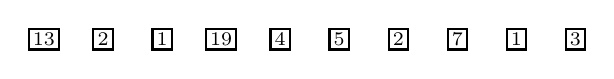
\begin{tikzpicture}
[-,thick,%
  every node/.style={shape=rectangle,inner sep=1.5pt,draw,thick},%
  scale=0.5]
\scriptsize
\foreach \xcoord/\xval in {
  0/13, 1.5/2, 3/1, 4.5/19, 6/4, 7.5/5, 9/2, 10.5/7, 12/1, 13.5/3}
{
  \node at (\xcoord,0) {$\xval$};
}
\end{tikzpicture}
}
%%
%%
\qquad
\subfigure[]{
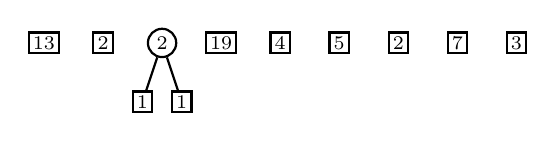
\begin{tikzpicture}
[-,thick,%
  every node/.style={shape=rectangle,inner sep=1.5pt,draw,thick},%
  scale=0.5]
\scriptsize
\node at (0,0) {$13$};
\node at (1.5,0) {$2$};
\node[shape=circle] at (3,0) {$2$}
  [sibling distance=1cm]
  child {node {$1$}}
  child {node {$1$}};
\node at (4.5,0) {$19$};
\node at (6,0) {$4$};
\node at (7.5,0) {$5$};
\node at (9,0) {$2$};
\node at (10.5,0) {$7$};
\node at (12,0) {$3$};
\end{tikzpicture}
}
%%
%%
\subfigure[]{
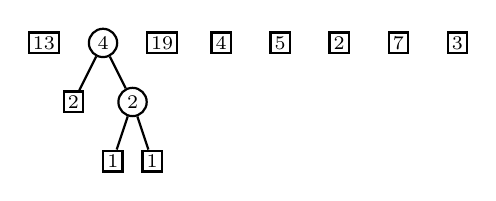
\begin{tikzpicture}
[-,thick,%
  every node/.style={shape=rectangle,inner sep=1.5pt,draw,thick},%
  scale=0.5]
\scriptsize
\node at (0,0) {$13$};
\node[shape=circle] at (1.5,0) {$4$}
  child {node {$2$}}
  child {node[shape=circle] {$2$}
    [sibling distance=1cm]
    child {node {$1$}}
    child {node {$1$}}};
\node at (3,0) {$19$};
\node at (4.5,0) {$4$};
\node at (6,0) {$5$};
\node at (7.5,0) {$2$};
\node at (9,0) {$7$};
\node at (10.5,0) {$3$};
\end{tikzpicture}
}
%%
%%
\qquad\qquad
\subfigure[]{
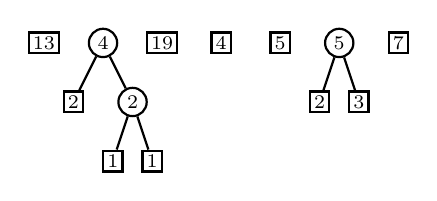
\begin{tikzpicture}
[-,thick,%
  every node/.style={shape=rectangle,inner sep=1.5pt,draw,thick},%
  scale=0.5]
\scriptsize
\node at (0,0) {$13$};
\node[shape=circle] at (1.5,0) {$4$}
  child {node {$2$}}
  child {node[shape=circle] {$2$}
    [sibling distance=1cm]
    child {node {$1$}}
    child {node {$1$}}};
\node at (3,0) {$19$};
\node at (4.5,0) {$4$};
\node at (6,0) {$5$};
\node[shape=circle] at (7.5,0) {$5$}
  [sibling distance=1cm]
  child {node {$2$}}
  child {node {$3$}};
\node at (9,0) {$7$};
\end{tikzpicture}
}
%%
%%
\subfigure[]{
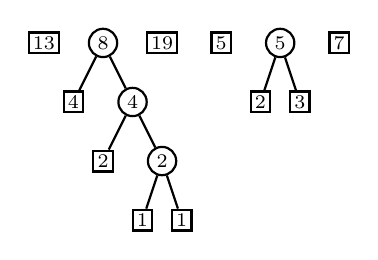
\begin{tikzpicture}
[-,thick,%
  every node/.style={shape=rectangle,inner sep=1.5pt,draw,thick},%
  scale=0.5]
\scriptsize
\node at (0,0) {$13$};
\node[shape=circle] at (1.5,0) {$8$}
  child {node {$4$}}
  child {node[shape=circle] {$4$}
    child {node {$2$}}
    child {node[shape=circle] {$2$}
      [sibling distance=1cm]
      child {node {$1$}}
      child {node {$1$}}}
  };
\node at (3,0) {$19$};
\node at (4.5,0) {$5$};
\node[shape=circle] at (6,0) {$5$}
  [sibling distance=1cm]
  child {node {$2$}}
  child {node {$3$}};
\node at (7.5,0) {$7$};
\end{tikzpicture}
}
%%
%%
\quad\qquad
\subfigure[]{
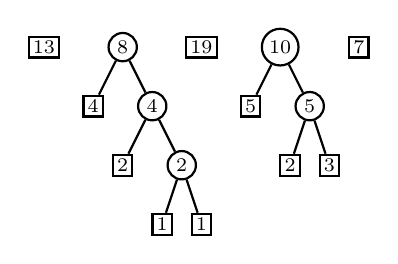
\begin{tikzpicture}
[-,thick,%
  every node/.style={shape=rectangle,inner sep=1.5pt,draw,thick},%
  scale=0.5]
\scriptsize
\node at (0,0) {$13$};
\node[shape=circle] at (2,0) {$8$}
  child {node {$4$}}
  child {node[shape=circle] {$4$}
    child {node {$2$}}
    child {node[shape=circle] {$2$}
      [sibling distance=1cm]
      child {node {$1$}}
      child {node {$1$}}}
  };
\node at (4,0) {$19$};
\node[shape=circle] at (6,0) {$10$}
  child {node {$5$}}
  child {node[shape=circle] {$5$}
    [sibling distance=1cm]
    child {node {$2$}}
    child {node {$3$}}
  };
\node at (8,0) {$7$};
\end{tikzpicture}
}
%%
%%
\qquad
\subfigure[]{
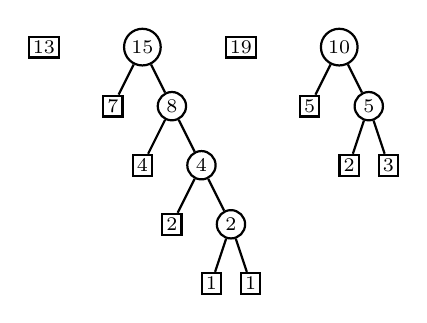
\begin{tikzpicture}
[-,thick,%
  every node/.style={shape=rectangle,inner sep=1.5pt,draw,thick},%
  scale=0.5]
\scriptsize
\node at (0,0) {$13$};
\node[shape=circle] at (2.5,0) {$15$}
  child {node {$7$}}
  child {node[shape=circle] {$8$}
    child {node {$4$}}
    child {node[shape=circle] {$4$}
      child {node {$2$}}
      child {node[shape=circle] {$2$}
        [sibling distance=1cm]
        child {node {$1$}}
        child {node {$1$}}}
    }
  };
\node at (5,0) {$19$};
\node[shape=circle] at (7.5,0) {$10$}
  child {node {$5$}}
  child {node[shape=circle] {$5$}
  [sibling distance=1cm]
    child {node {$2$}}
    child {node {$3$}}
  };
\end{tikzpicture}
}
%%
%%
\qquad\qquad
\subfigure[]{
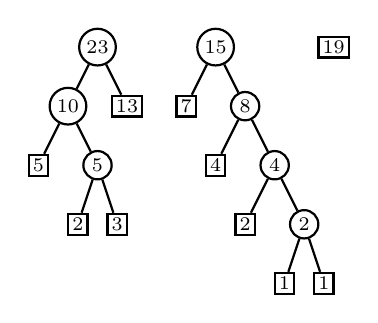
\begin{tikzpicture}
[-,thick,%
  every node/.style={shape=rectangle,inner sep=1.5pt,draw,thick},%
  scale=0.5]
\scriptsize
\node[shape=circle] at (0,0) {$23$}
  child {node[shape=circle] {$10$}
    child {node {$5$}}
    child {node[shape=circle] {$5$}
      [sibling distance=1cm]
      child {node {$2$}}
      child {node {$3$}}
    }
  }
  child {node {$13$}};
\node[shape=circle] at (3,0) {$15$}
  child {node {$7$}}
  child {node[shape=circle] {$8$}
    child {node {$4$}}
    child {node[shape=circle] {$4$}
      child {node {$2$}}
      child {node[shape=circle] {$2$}
        [sibling distance=1cm]
        child {node {$1$}}
        child {node {$1$}}}
    }
  };
\node at (6,0) {$19$};
\end{tikzpicture}
}
%%
%%
\qquad\quad
\subfigure[]{
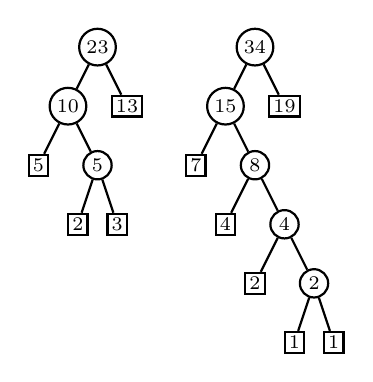
\begin{tikzpicture}
[-,thick,%
  every node/.style={shape=rectangle,inner sep=1.5pt,draw,thick},%
  scale=0.5]
\scriptsize
\node[shape=circle] at (0,0) {$23$}
  child {node[shape=circle] {$10$}
    child {node {$5$}}
    child {node[shape=circle] {$5$}
      [sibling distance=1cm]
      child {node {$2$}}
      child {node {$3$}}
    }
  }
  child {node {$13$}};
\node[shape=circle] at (4,0) {$34$}
  child {node[shape=circle] {$15$}
    child {node {$7$}}
    child {node[shape=circle] {$8$}
      child {node {$4$}}
      child {node[shape=circle] {$4$}
        child {node {$2$}}
        child {node[shape=circle] {$2$}
          [sibling distance=1cm]
          child {node {$1$}}
          child {node {$1$}}}
      }
    }
  }
  child {node {$19$}};
\end{tikzpicture}
}
%%
%%
\qquad\qquad
\subfigure[]{
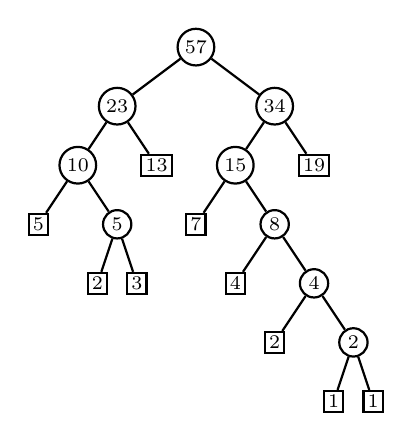
\begin{tikzpicture}
[-,thick,%
  every node/.style={shape=rectangle,inner sep=1.5pt,draw,thick},%
  scale=0.5]
\scriptsize
\node[shape=circle] {$57$}
  [sibling distance=4cm]
  child {node[shape=circle] {$23$}
    [sibling distance=2cm]
    child {node[shape=circle] {$10$}
      child {node {$5$}}
      child {node[shape=circle] {$5$}
        [sibling distance=1cm]
        child {node {$2$}}
        child {node {$3$}}
      }
    }
    child {node {$13$}}
  }
  child {node[shape=circle] {$34$}
    [sibling distance=2cm]
    child {node[shape=circle] {$15$}
      child {node {$7$}}
      child {node[shape=circle] {$8$}
        child {node {$4$}}
        child {node[shape=circle] {$4$}
          child {node {$2$}}
          child {node[shape=circle] {$2$}
            [sibling distance=1cm]
            child {node {$1$}}
            child {node {$1$}}}
        }
      }
    }
    child {node {$19$}}
  };
\end{tikzpicture}
}
\end{figure}

\end{document}

\caption{Constructing a Huffman tree.}
\label{fig:trees_forests:construct_Huffman_tree}
\end{figure}

The runtime analysis of
Algorithm~\ref{alg:trees_forests:binary_tree_Huffman_codes} depends on
the implementation of the priority\index{queue!priority} queue
$Q$. Suppose $Q$ is a simple unsorted list\index{list}. The
initialization on
line~\ref{alg:Huffman_tree:initialize_priority_queue} requires $O(n)$
time. The for loop from line~\ref{alg:Huffman_tree:for_loop:start}
to~\ref{alg:Huffman_tree:insert_into_queue} is executed exactly
$n - 1$ times. Searching $Q$ to determine the element of minimum
weight requires time at most $O(n)$. Determining two elements of
minimum weights requires time $O(2n)$. The for loop requires time
$O(2n^2)$, which is also the time requirement for the algorithm. An
efficient implementation of the priority queue $Q$, e.g. as a binary
minimum heap\index{heap!binary minimum}, can lower the running time of
Algorithm~\ref{alg:trees_forests:binary_tree_Huffman_codes} down to
$O(n \log_2(n))$.

Algorithm~\ref{alg:trees_forests:binary_tree_Huffman_codes} represents
the Huffman\index{Huffman code} code of an alphabet as a
binary\index{Huffman code!tree representation} tree $T$ rooted at
$r$. For an illustration of the process of constructing a Huffman
tree, see Figure~\ref{fig:trees_forests:construct_Huffman_tree}. To
determine the actual encoding of each symbol in the alphabet, we feed
$T$ and $r$ to
Algorithm~\ref{alg:trees_forests:Huffman_encoding_alphabet} to obtain
the encoding of each symbol. Starting from the root $r$ whose
designated label is the empty\index{string!empty} string
$\varepsilon$\index{$\varepsilon$}, the algorithm traverses the
vertices of $T$ in a breadth-first\index{breadth-first search} search
fashion. If $v$ is an internal vertex with label \tte, the label of
its left-child\index{child!left} is the concatenation \verb!e0! and
for the right-child\index{child!right} of $v$ we assign the label
\verb!e1!. If $v$ happens to be a leaf vertex, we take its label to be
its Huffman encoding. Any Huffman encoding assigned to a symbol of an
alphabet is not unique. Either of the two children of an internal
vertex can be designated as the left-~(respectively, right-)
child. The runtime of
Algorithm~\ref{alg:trees_forests:Huffman_encoding_alphabet} is
$O(|V|)$, where $V$ is the vertex set of $T$.

\begin{algorithm}[!htbp]
\index{Huffman code!encoding}
%%%%%%%%%%%%%%%%%%%%%%%%%%%%%%%%%%%%%%%%%%%%%%%%%%%%%%%%%%%%%%%%%%%%%%%%%%%
%% This file is part of the book
%%
%% Algorithmic Graph Theory
%% http://code.google.com/p/graph-theory-algorithms-book/
%%
%% Copyright (C) 2009--2011 Minh Van Nguyen <nguyenminh2@gmail.com>
%%
%% See the file COPYING for copying conditions.
%%%%%%%%%%%%%%%%%%%%%%%%%%%%%%%%%%%%%%%%%%%%%%%%%%%%%%%%%%%%%%%%%%%%%%%%%%%

\DontPrintSemicolon
\SetAlgoNoLine
%%
%% data section
\SetKwData{treeRoot}{root}
\SetKwData{one}{1}
\SetKwData{zero}{0}
%%
%% input
\KwIn{A binary tree $T$ representing the Huffman code of an alphabet
  $A$. The root $r$ of $T$.}
%%
%% output
\KwOut{A list $H$ representing a Huffman code of $A$, where $H[a_i]$
  corresponds to a Huffman encoding of $a_i \in A$.}
\BlankLine
%%
%% algorithm body
$H \assign [\,]$\tcc*[f]{list of Huffman encodings}\;
$Q \assign [r]$\tcc*[f]{queue of vertices}\;
\While{$\length(Q) > 0$}{
  $\treeRoot \assign \dequeue(Q)$\;
  \If{\rm \treeRoot is a leaf}{
    $H[\treeRoot] \assign$ label of \treeRoot\;
  }
  \Else{
    $a \assign$ left child of \treeRoot\;
    $b \assign$ right child of \treeRoot\;
    $\enqueue(Q, a)$\;
    $\enqueue(Q, b)$\;
    label of $a \assign$ label of \treeRoot $+$ \zero\;
    label of $b \assign$ label of \treeRoot $+$ \one\;
  }
}
\Return $H$\;

\caption{Huffman encoding of an alphabet.}
\label{alg:trees_forests:Huffman_encoding_alphabet}
\end{algorithm}

\begin{example}
Consider the alphabet $\cA = \{a, b, c, d, e, f\}$ with corresponding
weights $w(a) = 19$, $w(b) = 2$, $w(c) = 40$, $w(d) = 25$,
$w(e) = 31$, and $w(f) = 3$. Construct a binary tree representation of
the Huffman code of $\cA$ and determine the encoding of each symbol of
$\cA$.
\end{example}

\begin{proof}[Solution]
Use Algorithm~\ref{alg:trees_forests:binary_tree_Huffman_codes} to
construct a binary tree representation of the weighted alphabet
$\cA$. The resulting binary tree $T$ is shown in
Figure~\ref{fig:trees_forests:eg:binary_tree_Huffman_encodings:binary_tree},
where $a_i: w_i$ is an abbreviation for
``vertex $a_i$ has weight $w_i$''. The binary tree is rooted at
$k$. To encode each alphabetic symbol, input $T$ and $k$ into
Algorithm~\ref{alg:trees_forests:Huffman_encoding_alphabet} to get the
encodings shown in
Figure~\ref{fig:trees_forests:eg:binary_tree_Huffman_encodings:Huffman_encodings}.
\end{proof}

\begin{figure}[!htbp]
\centering
\index{Huffman code}
\index{Huffman code!tree representation}
%%%%%%%%%%%%%%%%%%%%%%%%%%%%%%%%%%%%%%%%%%%%%%%%%%%%%%%%%%%%%%%%%%%%%%%%%%%
%% This file is part of the book
%%
%% Algorithmic Graph Theory
%% http://code.google.com/p/graph-theory-algorithms-book/
%%
%% Copyright (C) 2009--2011 Minh Van Nguyen <nguyenminh2@gmail.com>
%%
%% See the file COPYING for copying conditions.
%%%%%%%%%%%%%%%%%%%%%%%%%%%%%%%%%%%%%%%%%%%%%%%%%%%%%%%%%%%%%%%%%%%%%%%%%%%

\documentclass{article}

\usepackage{subfigure}
\usepackage{tikz}
\usetikzlibrary{external}
\tikzexternalize{binary-tree-Huffman-encodings}

\begin{document}

\begin{figure}
\subfigure[]{
\label{fig:trees_forests:eg:binary_tree_Huffman_encodings:binary_tree}
\begin{tikzpicture}
[lineDecorate/.style={-,thick},%
  scale=1.5]
%% nodes or vertices
\foreach \nodename/\weight/\x/\y in {
  b/2/0/0, f/3/1/0, g/5/0.5/1, a/19/1.5/1, h/24/1/2, d/25/2/2,
  e/31/3/2, c/40/4/2, i/49/1.5/3, j/71/3.5/3, k/120/2.5/4}
{
  \node (\nodename) at (\x,\y) [] {\footnotesize$\nodename:\weight$};
}
%% edges or lines
\path
\foreach \startnode/\endnode in {
  g/b, g/f, h/g, h/a, i/h, i/d, j/e, j/c, k/i, k/j}
{
  (\startnode) edge[lineDecorate] node {} (\endnode)
};
\end{tikzpicture}
}
%%
%%
\subfigure[]{
\label{fig:trees_forests:eg:binary_tree_Huffman_encodings:Huffman_encodings}
\begin{tikzpicture}
[lineDecorate/.style={-,thick},%
  scale=1.5]
%% nodes or vertices
\foreach \nodename/\code/\x/\y in {
  b/0000/0/0, f/0001/1/0, g/000/0.5/1, a/001/1.5/1, h/00/1/2,
  d/01/2/2, e/10/3/2, c/11/4/2, i/0/1.5/3, j/1/3.5/3, k/$\varepsilon$/2.5/4}
{
  \node (\nodename) at (\x,\y) [] {\footnotesize$\texttt{\code}$};
}
%% edges or lines
\path
\foreach \startnode/\endnode in {
  g/b, g/f, h/g, h/a, i/h, i/d, j/e, j/c, k/i, k/j}
{
  (\startnode) edge[lineDecorate] node {} (\endnode)
};
\end{tikzpicture}
}
\end{figure}

\end{document}

\caption{Binary tree representation of an alphabet and its Huffman encodings.}
\label{fig:trees_forests:eg:binary_tree_Huffman_encodings}
\end{figure}


%%%%%%%%%%%%%%%%%%%%%%%%%%%%%%%%%%%%%%%%%%%%%%%%%%%%%%%%%%%%%%%%%%%%%%%%%%%

\section{Tree traversals}
\label{sec:trees_forests:tree_traversals}
\index{tree!traversal}

In computer\index{computer science} science,
\emph{tree traversal}\index{tree!traversal} refers to the process of
examining each vertex in a tree data structure. Starting at the root
of an ordered\index{tree!ordered} tree $T$, we can traverse the
vertices of $T$ in one of various ways.

A \emph{level-order traversal}\index{traversal!level-order} of an
ordered tree $T$ examines the vertices in increasing order of depth,
with vertices of equal depth being examined according to their
prescribed order. One way to think about
level-order\index{traversal!level-order} traversal is to consider
vertices of $T$ having the same depth as being ordered from left to
right in decreasing order of importance. If $[v_1, v_2, \dots, v_n]$
lists the vertices from left to right at depth $k$, a decreasing order
of importance can be realized by assigning each vertex a numeric label
using a labelling function $L: V(T) \to \R$ such that
$L(v_1) < L(v_2) < \cdots < L(v_n)$. In this way, a vertex with a
lower numeric label is examined prior to a vertex with a higher
numeric label. A level-order\index{traversal!level-order} traversal of
$T$, whose vertices of equal depth are prioritized according to $L$,
is an examination of the vertices of $T$ from top to bottom, left to
right. As an example, the level-order\index{traversal!level-order}
traversal of the tree in Figure~\ref{fig:trees_forests:tree_traversal}
is
\[
42,\, 4,\, 15,\, 2,\, 3,\, 5,\, 7,\, 10,\, 11,\, 12,\, 13,\, 14.
\]
Our discussion is formalized in
Algorithm~\ref{alg:trees_forests:level_order_traversal}, whose general
structure mimics that of breadth-first\index{breadth-first search}
search. For this reason, level-order traversal is also known as
\emph{breadth-first traversal}. Each vertex is
enqueued\index{queue!enqueue} and dequeued\index{queue!dequeue}
exactly once. The while loop is executed $n$ times, hence we have a
runtime of $O(n)$. Another name for level-order traversal is
\emph{top-down traversal} because we first visit the root node and
then work our way down the tree, increasing the depth as we move
downward.

\begin{figure}[!htbp]
\centering
\index{tree!traversal}
%%%%%%%%%%%%%%%%%%%%%%%%%%%%%%%%%%%%%%%%%%%%%%%%%%%%%%%%%%%%%%%%%%%%%%%%%%%
%% This file is part of the book
%%
%% Algorithmic Graph Theory
%% http://code.google.com/p/graph-theory-algorithms-book/
%%
%% Copyright (C) 2009--2011 Minh Van Nguyen <nguyenminh2@gmail.com>
%%
%% See the file COPYING for copying conditions.
%%%%%%%%%%%%%%%%%%%%%%%%%%%%%%%%%%%%%%%%%%%%%%%%%%%%%%%%%%%%%%%%%%%%%%%%%%%

\documentclass{article}

\usepackage{tikz}
\usetikzlibrary{external}
\usetikzlibrary{trees}
\tikzexternalize{tree-traversal}

\begin{document}

\begin{figure}
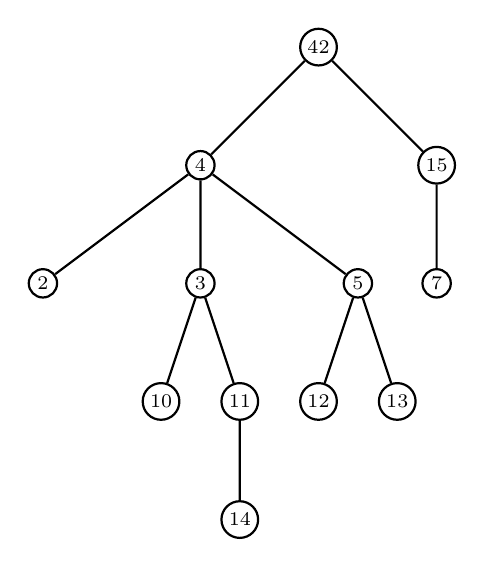
\begin{tikzpicture}
[-,thick,%
  every node/.style={shape=circle,inner sep=1.5pt,draw,thick}]
\scriptsize
\node {$42$}
  [sibling distance=3cm]
  child {node {$4$}
    [sibling distance=2cm]
    child {node {$2$}}
    child {node {$3$}
      [sibling distance=1cm]
      child {node {$10$}}
      child {node {$11$}
        child {node {$14$}}
      }
    }
    child {node {$5$}
      [sibling distance=1cm]
      child {node {$12$}}
      child {node {$13$}}
    }
  }
  child {node {$15$}
    [sibling distance=2cm]
    child {node {$7$}}
  };
\end{tikzpicture}
\end{figure}

\end{document}

\caption{Traversing a tree.}
\label{fig:trees_forests:tree_traversal}
\end{figure}

\begin{algorithm}[!htbp]
\index{traversal!level-order}
%%%%%%%%%%%%%%%%%%%%%%%%%%%%%%%%%%%%%%%%%%%%%%%%%%%%%%%%%%%%%%%%%%%%%%%%%%%
%% This file is part of the book
%%
%% Algorithmic Graph Theory
%% http://code.google.com/p/graph-theory-algorithms-book/
%%
%% Copyright (C) 2009, 2010 Minh Van Nguyen <nguyenminh2@gmail.com>
%%
%% See the file COPYING for copying conditions.
%%%%%%%%%%%%%%%%%%%%%%%%%%%%%%%%%%%%%%%%%%%%%%%%%%%%%%%%%%%%%%%%%%%%%%%%%%%

\DontPrintSemicolon
\SetAlgoNoLine
%%
%% data section
\SetKwInOut{Input}{Input}
\SetKwInOut{Output}{Output}
%%
%% input/output
\Input{An ordered tree $T$ on $n > 0$ vertices.}
\Output{A list of the vertices of $T$ in level-order.}
\BlankLine
%%
%% algorithm body
$L \assign [\,]$\;
$Q \assign$ empty queue\;
$r \assign$ root of $T$\;
$\enqueue(Q, r)$\;
\While{$\length(Q) > 0$}{
  $v \assign \dequeue(Q)$\;
  $\append(L, v)$\;
  $[u_1, u_2, \dots, u_k] \assign$ ordering of children of $v$\;
  \For{$i \assign 1, 2, \dots, k$}{
    $\enqueue(Q, u_i)$\;
  }
}
\Return $L$\;

\caption{Level-order traversal.}
\label{alg:trees_forests:level_order_traversal}
\end{algorithm}

\emph{Pre-order traversal}\index{traversal!pre-order} is a traversal
of an ordered tree using a general strategy similar to
depth-first\index{depth-first search} search. For this reason,
pre-order\index{traversal!pre-order} traversal is also referred to as
\emph{depth-first traversal}. Parents are visited prior to their
respective children and siblings are visited according to their
prescribed order. The pseudocode for
pre-order\index{traversal!pre-order} traversal is presented in
Algorithm~\ref{alg:trees_forests:pre_order_traversal}. Note the
close resemblance to
Algorithm~\ref{alg:trees_forests:level_order_traversal}; the only
significant change is to use a stack\index{stack} instead of a
queue\index{queue}. Each vertex is pushed\index{stack!push} and
popped\index{stack!pop} exactly once, so the while loop is executed
$n$ times, resulting in a runtime of $O(n)$. Using
Algorithm~\ref{alg:trees_forests:pre_order_traversal}, a
pre-order\index{traversal!pre-order} traversal of the tree in
Figure~\ref{fig:trees_forests:tree_traversal} is
\[
42,\, 4,\, 2,\, 3,\, 10,\, 11,\, 14,\, 5,\, 12,\, 13,\, 15,\, 7.
\]

\begin{algorithm}[!htbp]
\index{traversal!pre-order}
%%%%%%%%%%%%%%%%%%%%%%%%%%%%%%%%%%%%%%%%%%%%%%%%%%%%%%%%%%%%%%%%%%%%%%%%%%%
%% This file is part of the book
%%
%% Algorithmic Graph Theory
%% http://code.google.com/p/graph-theory-algorithms-book/
%%
%% Copyright (C) 2009, 2010, 2011 Minh Van Nguyen <nguyenminh2@gmail.com>
%%
%% See the file COPYING for copying conditions.
%%%%%%%%%%%%%%%%%%%%%%%%%%%%%%%%%%%%%%%%%%%%%%%%%%%%%%%%%%%%%%%%%%%%%%%%%%%

\DontPrintSemicolon
\SetAlgoNoLine
%%
%% data section
\SetKwInOut{Input}{Input}
\SetKwInOut{Output}{Output}
%%
%% input/output
\Input{An ordered tree $T$ on $n > 0$ vertices.}
\Output{A list of the vertices of $T$ in pre-order.}
\BlankLine
%%
%% algorithm body
$L \assign [\,]$\;
$S \assign$ empty stack\;
$r \assign$ root of $T$\;
$\push(S, r)$\;
\While{$\length(S) > 0$}{
  $v \assign \pop(S)$\;
  $\append(L, v)$\;
  $[u_1, u_2, \dots, u_k] \assign$ ordering of children of $v$\;
  \For{$i \assign k, k-1, \dots, 1$}{
    $\push(S, u_i)$\;
  }
}
\Return $L$\;

\caption{Pre-order traversal.}
\label{alg:trees_forests:pre_order_traversal}
\end{algorithm}

Whereas pre-order traversal lists a vertex $v$ the first time we visit
it, \emph{post-order traversal}\index{traversal!post-order} lists $v$
the last time we visit it. In other words, children are visited prior
to their respective parents, with siblings being visited in their
prescribed order. The prefix ``pre'' in ``pre-order traversal'' means
``before'', i.e. visit parents before visiting children. On the other
hand, the prefix ``post'' in ``post-order traversal'' means ``after'',
i.e. visit parents after having visited their children. The pseudocode
for post-order\index{traversal!post-order} traversal is presented in
Algorithm~\ref{alg:trees_forests:post_order_traversal}, whose general
structure bears close resemblance to
Algorithm~\ref{alg:trees_forests:pre_order_traversal}. The while loop
of the former is executed $n$ times because each vertex is
pushed\index{stack!push} and popped\index{stack!pop} exactly once,
resulting in a runtime of $O(n)$. The
post-order\index{traversal!post-order} traversal of the tree in
Figure~\ref{fig:trees_forests:tree_traversal} is
\[
2,\, 10,\, 14,\, 11,\, 3,\, 12,\, 13,\, 5,\, 4,\, 7,\, 15,\, 42.
\]

\begin{algorithm}[!htbp]
\index{traversal!post-order}
\input{algorithm/trees-forests/post-order-traversal.tex}
\caption{Post-order traversal.}
\label{alg:trees_forests:post_order_traversal}
\end{algorithm}

Instead of traversing a tree $T$ from top to bottom as is the case
with level-order\index{traversal!level-order} traversal, we can
reverse the direction of our traversal by traversing a tree from
bottom to top. Called
\emph{bottom-up traversal}\index{traversal!bottom-up}, we first visit
all the leaves of $T$ and consider the subtree\index{subtree} $T_1$
obtained by vertex\index{vertex!deletion} deletion of those
leaves\index{vertex!leaf}. We then recursively\index{recursion} perform
bottom-up\index{traversal!bottom-up} traversal of $T_1$ by visiting
all of its leaves and obtain the subtree $T_2$ resulting from
vertex\index{vertex!deletion} deletion of those leaves of $T_1$. Apply
bottom-up\index{traversal!bottom-up} traversal to $T_2$ and its vertex
deletion subtrees until we have visited all vertices, including the
root vertex. The result is a procedure for bottom-up traversal as
presented in Algorithm~\ref{alg:trees_forests:bottom_up_traversal}. In
lines~\ref{alg:bottom_up_traversal:children_count}
to~\ref{alg:bottom_up_traversal:children_count_end}, we initialize the
list $C$ to contain the number of children of vertex $i$. This takes
$O(m)$ time, where $m =
|E(T)|$. Lines~\ref{alg:bottom_up_traversal:empty_queue_R}
to~\ref{alg:bottom_up_traversal:enqueue_R_w} extract all the leaves
of $T$ and add them to the queue $Q$. From
lines~\ref{alg:bottom_up_traversal:empty_list_L}
to~\ref{alg:bottom_up_traversal:enqueue_Q_u}, we repeatedly apply
bottom-up\index{traversal!bottom-up} traversal to subtrees of $T$. As
each vertex is enqueued\index{queue!enqueue} and
dequeued\index{queue!dequeue} exactly once, the two loops together run
in time $O(n)$ and therefore
Algorithm~\ref{alg:trees_forests:bottom_up_traversal} has a runtime of
$O(n + m)$. As an example, a bottom-up\index{traversal!bottom-up}
traversal of the tree in Figure~\ref{fig:trees_forests:tree_traversal}
is
\[
2,\, 7,\, 10,\, 12,\, 13,\, 14,\, 15,\, 5,\, 11,\, 3,\, 4,\, 42.
\]

\begin{algorithm}[!htbp]
\index{traversal!bottom-up}
%%%%%%%%%%%%%%%%%%%%%%%%%%%%%%%%%%%%%%%%%%%%%%%%%%%%%%%%%%%%%%%%%%%%%%%%%%%
%% This file is part of the book
%%
%% Algorithmic Graph Theory
%% http://code.google.com/p/graph-theory-algorithms-book/
%%
%% Copyright (C) 2009, 2010 Minh Van Nguyen <nguyenminh2@gmail.com>
%%
%% See the file COPYING for copying conditions.
%%%%%%%%%%%%%%%%%%%%%%%%%%%%%%%%%%%%%%%%%%%%%%%%%%%%%%%%%%%%%%%%%%%%%%%%%%%

\DontPrintSemicolon
\SetAlgoNoLine
%%
%% data section
\SetKwInOut{Input}{Input}
\SetKwInOut{Output}{Output}
%%
%% input/output
\Input{An ordered tree $T$ on $n > 0$ vertices.}
\Output{A list of the vertices of $T$ in bottom-up order.}
\BlankLine
%%
%% algorithm body
$Q \assign$ empty queue\;
$r \assign$ root of $T$\;
$C \assign [0, 0, \dots, 0]$\tcc*[f]{$n$ copies of $0$}\;
\For{\rm each edge $(u,v) \in E(T)$}{
  $C[u] \assign C[u] + 1$\;
}
$R \assign$ empty queue\;
$\enqueue(R, r)$\;
\While{$\length(R) > 0$}{
  $v \assign \dequeue(R)$\;
  \For{\rm each $w \in \children(v)$}{
    \eIf{$C[w] = 0$}{
      $\enqueue(Q, w)$\;
    }{
      $\enqueue(R, w)$\;
    }
  }
}
$L \assign [\,]$\;
\While{$\length(Q) > 0$}{
  $v \assign \dequeue(Q)$\;
  $\append(L, v)$\;
  \If{$v \neq r$}{
    $C[\parent(v)] \assign C[\parent(v)] - 1$\;
    \If{$C[\parent(v)] = 0$}{
      $u \assign \parent(v)$\;
      $\enqueue(Q, u)$\;
    }
  }
}
\Return $L$\;

\caption{Bottom-up traversal.}
\label{alg:trees_forests:bottom_up_traversal}
\end{algorithm}

\begin{algorithm}[!htbp]
\index{traversal!in-order}
%%%%%%%%%%%%%%%%%%%%%%%%%%%%%%%%%%%%%%%%%%%%%%%%%%%%%%%%%%%%%%%%%%%%%%%%%%%
%% This file is part of the book
%%
%% Algorithmic Graph Theory
%% http://code.google.com/p/graph-theory-algorithms-book/
%%
%% Copyright (C) 2009--2011 Minh Van Nguyen <nguyenminh2@gmail.com>
%%
%% See the file COPYING for copying conditions.
%%%%%%%%%%%%%%%%%%%%%%%%%%%%%%%%%%%%%%%%%%%%%%%%%%%%%%%%%%%%%%%%%%%%%%%%%%%

\DontPrintSemicolon
\SetAlgoNoLine
%%
%% data section
\SetKwData{MyTrue}{True}
\SetKwData{NULL}{\footnotesize{NULL}}
%%
%% input
\KwIn{A binary tree $T$ on $n > 0$ vertices.}
%%
%% output
\KwOut{A list of the vertices of $T$ in in-order.}
\BlankLine
%%
%% algorithm body
$L \assign [\,]$\;
$S \assign$ empty stack\;
$v \assign$ root of $T$\;
\While{$\MyTrue$}{
  \If{$v \neq \NULL$}{
    $\push(S, v)$\;
    $v \assign$ left-child of $v$\;
  }
  \Else{
    \If{$\length(S) = 0$}{
      exit the loop\;
    }
    $v \assign \pop(S)$\;
    $\append(L, v)$\;
    $v \assign$ right-child of $v$\;
  }
}
\Return $L$\;

\caption{In-order traversal.}
\label{alg:trees_forests:in_order_traversal}
\end{algorithm}

Yet another common tree traversal technique is called
\emph{in-order traversal}\index{traversal!in-order}. However, in-order
traversal is only applicable to binary\index{tree!binary} trees,
whereas the other traversal techniques we considered above can be
applied to any tree with at least one vertex. Given a binary tree $T$
having at least one vertex, in-order traversal first visits the root
of $T$ and consider its left-\index{child!left} and
right-children\index{child!right}. We then
recursively\index{recursion} apply in-order\index{traversal!in-order}
traversal to the left\index{subtree!left} and
right\index{subtree!right} subtrees of the root vertex. Notice the
symmetry in our description of in-order\index{traversal!in-order}
traversal: start at the root, then traverse the left and right
subtrees in in-order. For this reason, in-order traversal is sometimes
referred to as \emph{symmetric traversal}. Our discussion is
summarized in Algorithm~\ref{alg:trees_forests:in_order_traversal}.
In the latter algorithm, if a vertex does not have a left-child, then
the operation of finding its left-child returns \texttt{NULL}. The
same holds when the vertex does not have a right-child. Since each
vertex is pushed\index{stack!push} and popped\index{stack!pop} exactly
once, it follows that in-order traversal runs in time $O(n)$. Using
Algorithm~\ref{alg:trees_forests:in_order_traversal}, an in-order
traversal of the tree in
Figure~\ref{fig:trees_forests:eg:binary_tree_Huffman_encodings:Huffman_encodings}
is
\[
\texttt{0000},\, \texttt{000},\, \texttt{0001},\, \texttt{00},\,
\texttt{001}, \texttt{0},\, \texttt{01},\, \varepsilon,\,
\texttt{10},\, \texttt{1},\texttt{11}.
\]


%%%%%%%%%%%%%%%%%%%%%%%%%%%%%%%%%%%%%%%%%%%%%%%%%%%%%%%%%%%%%%%%%%%%%%%%%%%

\section{Problems}

\begin{quote}
\footnotesize
When solving problems, dig at the roots instead of just hacking at the
leaves. \\
\noindent
--- Anthony J. D'Angelo\index{D'Angelo, Anthony J.},
\emph{The College Blue Book}
\end{quote}

\begin{problem}
\item Construct all nonisomorphic trees of order $7$.

\item Let $G$ be a weighted connected graph and let $T$ be a subgraph
  of $G$. Then $T$ is a
  \emph{maximum spanning tree}\index{spanning tree!maximum} of $G$
  provided that the following conditions are satisfied:
  %%
  \begin{enumerate}[(a)]
  \item $T$ is a spanning tree of $G$.

  \item The total weight of $T$ is maximum among all spanning trees of
    $G$.
  \end{enumerate}
  %%
  Modify Kruskal's\index{Kruskal!algorithm},
  Prim's\index{Prim!algorithm}, and
  Bor\r{u}vka's\index{Bor\r{u}vka!algorithm} algorithms to return a
  maximum spanning tree of $G$.

\item Describe and present pseudocode of an algorithm to construct all
  spanning trees of a connected graph. What is the worst-case runtime
  of your algorithm? How many of the constructed spanning trees are
  nonisomorphic to each other? Repeat the exercise for minimum and
  maximum spanning trees.

\item Consider an undirected, connected simple graph $G = (V,E)$ of
  order $n$ and size $m$ and having an integer weight function
  $w: E \to \Z$ given by $w(e) > 0$ for all $e \in E$. Suppose that
  $G$ has $N$ minimum spanning trees.\index{Yamada, Takeo}
  Yamada\index{Kataoka, Seiji}~et~al.~\cite{YamadaEtAl2010} provide an
  $O(Nm \ln n)$ algorithm to construct all the $N$ minimum spanning
  trees of $G$. Describe and provide pseudocode of the
  Yamada-Kataoka-Watanabe\index{Watanabe, Kohtaro} algorithm. Provide
  runtime analysis and prove the correctness of this algorithm.

\item\label{prob:trees_forests:binary_tree_test} The solution of
  Example~\ref{eg:trees_forests:branch_cut_binary_tree} relied on the
  following result: Let $T = (V,E)$ be a tree rooted at $v_0$ and
  suppose $v_0$ has exactly two children. If
  $\max_{v \in V} \deg(v) = 3$ and $v_0$ is the only vertex with
  degree $2$, then $T$ is a binary tree. Prove this statement. Give
  examples of graphs that are binary trees but do not satisfy the
  conditions of the result. Under which conditions would the above
  test return an incorrect answer?

\item What is the worst-case runtime of
  Algorithm~\ref{alg:trees_forests:randomized_spanning_tree_construction}?

\item Figure~\ref{fig:trees_forests:grid_graph_spanning_trees} shows
  two nonisomorphic spanning trees of the $4 \times 4$ grid graph.
  %%
  \begin{enumerate}[(a)]
  \item For each $n = 1, 2, \dots, 7$, construct all nonisomorphic
    spanning trees of the $n \times n$ grid graph.

  \item Explain and provide pseudocode of an algorithm for
    constructing all spanning\index{spanning tree} trees of the
    $n \times n$ grid\index{grid!graph} graph, where $n > 0$.

  \item In general, if $n$ is a positive integer, how many
    nonisomorphic spanning trees are there in the $n \times n$ grid
    graph?

  \item Describe and provide pseudocode of an algorithm to generate a
    random\index{algorithm!random} spanning tree\index{spanning tree}
    of the $n \times n$ grid graph. What is the worst-case runtime of
    your algorithm?
  \end{enumerate}

\item Theorem~\ref{thm:trees_forests:recursive_construction_trees}
  shows how to recursively\index{recursion} construct a new tree from
  a given collection of trees, hence it can be considered as a
  recursive\index{tree!recursive definition} definition of trees. To
  prove theorems based upon recursive definitions, we use a proof
  technique called
  \emph{structural induction}\index{induction!structural}. Let $S(C)$
  be a statement about the collection of structures $C$, each of which
  is defined by a recursive definition. In the base case, prove $S(C)$
  for the basis structure(s) $C$. For the inductive\index{induction}
  case, let $X$ be a structure formed using the recursive definition
  from the structures $Y_1, Y_2, \dots, Y_k$. Assume for induction
  that the statements $S(Y_1),\, S(Y_2), \dots, S(Y_k)$ hold and use
  the inductive hypotheses $S(Y_i)$ to prove $S(X)$. Hence conclude
  that $S(X)$ is true for all $X$. Apply structural induction to show
  that any graph constructed using
  Theorem~\ref{thm:trees_forests:recursive_construction_trees} is
  indeed a tree.

\item In Kruskal's\index{Kruskal!algorithm}
  Algorithm~\ref{alg:trees_forests:Kruskal_algorithm},
  line~\ref{alg:Kruskal:edge_not_in_T_acyclic} requires that the
  addition of a new edge to $T$ does not result in $T$ having a
  cycle. A tree by definition has no cycles. Suppose
  line~\ref{alg:Kruskal:edge_not_in_T_acyclic} is changed to:
  \[
  \textbf{if } e_i \notin E(T)
  \text{ and }
  T \cup \{e_i\} \text{ is a tree } \textbf{then}
  \]
  With this change, explain why
  Algorithm~\ref{alg:trees_forests:Kruskal_algorithm} would return a
  minimum spanning tree or why the algorithm would fail to do so.

\item This problem is concerned with improving the runtime of
  Kruskal's\index{Kruskal!algorithm}
  Algorithm~\ref{alg:trees_forests:Kruskal_algorithm}. Explain how to
  use a priority queue to obviate the need for sorting the edges by
  weight. Investigate the union-find\index{union-find} data
  structure. Explain how to use union-find to ensure that the addition
  of each edge results in an acyclic\index{acyclic} graph.

\item Figure~\ref{fig:trees_forests:weighted_Chvatal_graph} shows a
  weighted version of the Chv\'atal\index{Chv\'atal graph} graph,
  which has $12$ vertices and $24$ edges. Use this graph as input to
  Kruskal's\index{Kruskal!algorithm},
  Prim's\index{Prim!algorithm}, and
  Bor\r{u}vka's\index{Bor\r{u}vka!algorithm} algorithms and compare
  the resulting minimum\index{spanning tree!minimum} spanning trees.

\begin{figure}[!htbp]
\centering
\index{Chv\'atal graph}
%%%%%%%%%%%%%%%%%%%%%%%%%%%%%%%%%%%%%%%%%%%%%%%%%%%%%%%%%%%%%%%%%%%%%%%%%%%
%% This file is part of the book
%%
%% Algorithmic Graph Theory
%% http://code.google.com/p/graph-theory-algorithms-book/
%%
%% Copyright (C) 2009--2011 Minh Van Nguyen <nguyenminh2@gmail.com>
%%
%% See the file COPYING for copying conditions.
%%%%%%%%%%%%%%%%%%%%%%%%%%%%%%%%%%%%%%%%%%%%%%%%%%%%%%%%%%%%%%%%%%%%%%%%%%%

\documentclass{article}

\usepackage{tikz}
\usepackage{tkz-berge}  %% for drawing combinatorial graphs
\usetikzlibrary{external}
\tikzexternalize{weighted-Chvatal-graph}

\begin{document}

\begin{figure}
\begin{tikzpicture}
[lineDecorate/.style={-,thick},%
  nodeDecorate/.style={shape=circle,inner sep=1.5pt,draw,thick},%
  scale=3]
\scriptsize
%% nodes or vertices
\foreach \nodename/\x/\y in {
  %% inner star
  5/0.0/1.0, 9/0.9510/0.3090, 8/0.5877/-0.8090, 7/-0.5877/-0.8090,
  6/-0.9510/0.3090,
  %% outer pentagon
  0/0.0/2.0, 4/1.9021/0.6180, 3/1.1755/-1.6180, 2/-1.1755/-1.6180,
  1/-1.9021/0.6180,
  %% inner two nodes
  10/0.5/-0.2, 11/-0.5/-0.2}
{
  \node (\nodename) at (\x,\y) [nodeDecorate] {\scriptsize$\nodename$};
}
%% edges or lines
\tikzstyle{EdgeStyle}=[-,thick]
\tikzstyle{LabelStyle}=[fill=white]
\foreach \startnode/\endnode/\bend/\weight in {
  0/1/bend right/11.4, 0/4/bend left/40.7, 0/6/bend right/17.1,
  0/9/bend left/14.4, 1/2/bend right/6.9, 1/5/bend left/5.6,
  1/7/bend right/0.2, 2/3/bend right/44.2, 2/6/bend left/43.2,
  2/8/bend right/22, 3/4/bend right/42.7, 3/7/bend left/36.6,
  3/9/bend right/10.2, 4/5/bend right/35.4, 4/8/bend left/9.1,
  5/10/bend left/15, 5/11/bend right/14.5, 6/10/bend left=0/8.5,
  6/11/bend left=0/11.8, 7/8/bend left=0/22.1, 7/11/bend left=0/27.1,
  8/10/bend left=0/17, 9/10/bend left=0/3.7, 9/11/bend left=0/48}
{
  \Edge[label=$\weight$,style=\bend](\startnode)(\endnode)
}
\end{tikzpicture}
\end{figure}

\end{document}

\caption{Weighted Chv\'atal graph.}
\label{fig:trees_forests:weighted_Chvatal_graph}
\end{figure}

\item Algorithm~\ref{alg:trees_forests:randomized_spanning_tree_construction}
  presents a randomized procedure to construct a
  spanning\index{spanning tree!randomized construction} tree of a
  given connected graph via repeated edge deletion.
  %%
  \begin{enumerate}[(a)]
  \item Describe and present pseudocode of a
    randomized\index{algorithm!random} algorithm to \emph{grow} a
    spanning tree via edge addition.

  \item Would
    Algorithm~\ref{alg:trees_forests:randomized_spanning_tree_construction}
    still work if the input graph $G$ has self-loops or multiple
    edges? Explain why or why not. If not, modify
    Algorithm~\ref{alg:trees_forests:randomized_spanning_tree_construction}
    to handle the case where $G$ has self-loops and multiple edges.

  \item Repeat the previous exercise for
    Kruskal's\index{Kruskal!algorithm},
    Prim's\index{Prim!algorithm}, and
    Bor\r{u}vka's\index{Bor\r{u}vka!algorithm} algorithms.
  \end{enumerate}

\begin{algorithm}[!htbp]
\index{algorithm!random}
\index{complete graph}
\index{spanning tree!randomized construction}
%%%%%%%%%%%%%%%%%%%%%%%%%%%%%%%%%%%%%%%%%%%%%%%%%%%%%%%%%%%%%%%%%%%%%%%%%%%
%% This file is part of the book
%%
%% Algorithmic Graph Theory
%% http://code.google.com/p/graph-theory-algorithms-book/
%%
%% Copyright (C) 2009, 2010, 2011 Minh Van Nguyen <nguyenminh2@gmail.com>
%%
%% See the file COPYING for copying conditions.
%%%%%%%%%%%%%%%%%%%%%%%%%%%%%%%%%%%%%%%%%%%%%%%%%%%%%%%%%%%%%%%%%%%%%%%%%%%

\DontPrintSemicolon
\SetAlgoNoLine
%%
%% data section
\SetKwInOut{Input}{Input}
\SetKwInOut{Output}{Output}
%%
%% input/output
\Input{A positive integer $n$ representing the order of $K_n$, with
  vertex set $V = \{0, 1, \dots, n-1\}$.}
\Output{A random spanning tree of $K_n$.}
\BlankLine
%%
%% algorithm body
\If{$n = 1$}{
  \Return $K_1$\;
}
$P \assign$ random permutation of $V$\;
$T \assign$ null tree\;
\For{$i \assign 1, 2, \dots, n-1$}{
  $j \assign$ random element from $\{0, 1, \dots, i-1\}$\;
  add edge $(P[j],\, P[i])$ to $T$\;
}
\Return $T$\;

\caption{Random spanning tree of $K_n$.}
\label{alg:trees_forests:random_spanning_tree_K_n}
\end{algorithm}

\item Algorithm~\ref{alg:trees_forests:random_spanning_tree_K_n}
  constructs a random spanning tree of the complete graph $K_n$ on
  $n > 0$ vertices. Its runtime is dependent on efficient algorithms
  for obtaining a random permutation of a set of objects, and choosing
  a random element from a given set.
  %%
  \begin{enumerate}[(a)]
  \item Describe and analyze the runtime of a procedure to construct a
    random permutation\index{permutation!random} of a set of
    nonnegative integers.

  \item Describe an algorithm for randomly choosing an element of a
    set of nonnegative integers. Analyze the runtime of this
    algorithm.

  \item Taking into consideration the previous two algorithms, what is
    the runtime of
    Algorithm~\ref{alg:trees_forests:random_spanning_tree_K_n}?
  \end{enumerate}

\item We want to generate a random\index{algorithm!random} undirected,
  connected simple\index{simple graph} graph on $n$ vertices and
  having $m$ edges. Start by generating a random
  spanning\index{spanning tree} tree $T$ of
  $K_n$\index{complete graph}. Then add random edges to $T$ until the
  requirements are satisfied.
  %%
  \begin{enumerate}[(a)]
  \item Present pseudocode to realize the above procedure. What is the
    worst-case runtime of your algorithm?

  \item Modify your algorithm to handle the case where $m < n-1$. Why
    must $m \geq n-1$?

  \item Modify your algorithm to handle the case where each edge has a
    weight within the closed interval $[\alpha, \beta]$.
  \end{enumerate}

\item Enumerate all the different binary\index{binary tree} trees on
  $5$ vertices.

\item Algorithm~\ref{alg:trees_forests:random_binary_tree} generates a
  random\index{algorithm!random} binary\index{binary tree!random} tree
  on $n > 0$ vertices. Modify this algorithm so that it generates a
  random $k$-ary tree of order $n > 0$, where $k \geq 3$.

\item Show by giving an example that the Morse\index{Morse code} code
  is not prefix-free\index{code!prefix-free}.

\item Consider the alphabet $\cA = \{a,b,c\}$ with corresponding
  probabilities~(or weights) $p(a) = 0.5$, $p(b) = 0.3$, and
  $p(c) = 0.2$. Generate two different Huffman\index{Huffman code}
  codes for $\cA$ and illustrate the tree representations of those
  codes.

\item Find the Huffman\index{Huffman code} code for the letters of the
  English\index{alphabet!English} alphabet weighted by the frequency
  of common American usage.\footnote{
    You can find this on the Internet or in the literature. Part of
    this exercise is finding this frequency distribution yourself.
  }

\item Let $G = (V_1, E_2)$ be a graph and $T = (V_2, E_2)$ a spanning
  tree of $G$. Show that there is a one-to-one correspondence between
  fundamental\index{cycle!fundamental} cycles in $G$ and edges not in
  $T$.

\item Let $G = (V,E)$ be the $3 \times 3$ grid\index{grid!graph} graph
  and $T_1 = (V_1, E_1)$, $T_2 = (V_2, E_2)$ be spanning trees of $G$
  in Example~\ref{eg:trees_forests:spanning_tree}. Find a fundamental
  cycle in $G$ for $T_1$ that is not a fundamental cycle in $G$ for
  $T_2$.

\item Usually there exist many spanning trees of a graph. Classify
  those graphs for which there is only one spanning tree. In other
  words, find necessary and sufficient conditions for a graph $G$ such
  that if $T$ is a spanning tree of $G$ then $T$ is unique.

\item Convert the function \texttt{graycodeword} into a pure Python
  function.

\item Example~\ref{eg:trees_forests:Euler_phi_function_tree} verifies
  that for any positive integer $n > 1$, repeated iteration of the
  Euler\index{Euler!phi function} phi function $\varphi(n)$ eventually
  produces $1$. Show that this is the case or provide an explanation
  why it is in general false.

\item The Collatz\index{Collatz!conjecture}
  conjecture~\cite{Lagarias1985} asserts that for any integer $n > 0$,
  repeated iteration of the function
  \[
  T(n)
  =
  \begin{cases}
  \frac{3n + 1}{2}, & \text{if $n$ is odd}, \\[4pt]
  \frac{n}{2}, & \text{if $n$ is even}
  \end{cases}
  \]
  eventually produces the value $1$. For example, repeated iteration
  of $T(n)$ starting from $n = 22$ results in the sequence
  %%
  \begin{equation}
  \label{eqn:trees_forests:Collatz_sequence_22}
  22,\, 11,\, 17,\, 26,\, 13,\, 20,\, 10,\, 5,\, 8,\, 4,\, 2,\, 1.
  \end{equation}
  %%
  One way to think about the Collatz\index{Collatz!conjecture}
  conjecture is to consider the digraph $G$ produced by considering
  $(a_i,\, T(a_i))$ as a directed edge of $G$. Then the Collatz
  conjecture can be rephrased to say that there is some integer
  $k > 0$ such that $(a_k,\, T(a_k)) = (2, 1)$ is a directed edge of
  $G$. The graph obtained in this manner is called the
  \emph{Collatz graph}\index{Collatz!graph} of $T(n)$. Given a
  collection of positive integers
  $\alpha_1, \alpha_2, \dots, \alpha_k$, let $G_{\alpha_i}$ be the
  Collatz graph of the function $T(\alpha_i)$ with initial iteration
  value $\alpha_i$. Then the union of the $G_{\alpha_i}$ is the
  directed tree
  \[
  \bigcup_i G_{\alpha_i}
  \]
  rooted at $1$, called the \emph{Collatz tree}\index{Collatz!tree} of
  $(\alpha_1, \alpha_2, \dots, \alpha_k)$.
  Figure~\ref{fig:trees_forests:Collatz_graph_union} shows such a tree
  for the collection of initial iteration values $1024$, $336$, $340$,
  $320$, $106$, $104$, and $96$. See
  Lagarias\index{Lagarias, Jeffrey C.}~\cite{Lagarias2009a,Lagarias2009b}
  for a comprehensive survey of the Collatz\index{Collatz!conjecture}
  conjecture.
  %%
  \begin{enumerate}[(a)]
  \item The \emph{Collatz sequence}\index{Collatz!sequence} of a
    positive integer $n > 1$ is the integer sequence produced by
    repeated iteration of $T(n)$ with initial iteration value $n$. For
    example, the Collatz sequence of $n = 22$ is the
    sequence~\eqref{eqn:trees_forests:Collatz_sequence_22}. Write a
    Sage function to produce the Collatz sequence of an integer $n > 1$.

  \item The \emph{Collatz length}\index{Collatz!length} of $n > 1$ is
    the number of terms in the Collatz sequence of $n$, inclusive of
    the starting iteration value and the final integer $1$. For
    instance, the Collatz length of $22$ is $12$, that of $106$ is
    $11$, and that of $51$ is $18$. Write a Sage function to compute
    the Collatz length of a positive integer $n > 1$. If $n > 1$ is a
    vertex in a Collatz tree, verify that the Collatz length of $n$ is
    the distance $d(n,1)$.

  \item Describe the Collatz\index{Collatz!graph} graph produced by
    the function $T(n)$ with initial iteration value $n = 1$.

  \item Fix a positive integer $n > 1$ and let $L_i$ be the Collatz
    length of the integer $1 \leq i \leq n$. Plot the pairs $(i, L_i)$
    on one set of axes.
  \end{enumerate}

\begin{figure}[!htbp]
\centering
\index{Collatz!graph}
\index{Collatz!tree}
%%%%%%%%%%%%%%%%%%%%%%%%%%%%%%%%%%%%%%%%%%%%%%%%%%%%%%%%%%%%%%%%%%%%%%%%%%%
%% This file is part of the book
%%
%% Algorithmic Graph Theory
%% http://code.google.com/p/graph-theory-algorithms-book/
%%
%% Copyright (C) 2009--2011 Minh Van Nguyen <nguyenminh2@gmail.com>
%%
%% See the file COPYING for copying conditions.
%%%%%%%%%%%%%%%%%%%%%%%%%%%%%%%%%%%%%%%%%%%%%%%%%%%%%%%%%%%%%%%%%%%%%%%%%%%

\documentclass{article}

\usepackage{tikz}
\usetikzlibrary{external}
\usetikzlibrary{trees}
\tikzexternalize{collatz-graph-union}

\begin{document}

\begin{figure}
\begin{tikzpicture}
[<-,>=stealth,thick]
\footnotesize
\node {$1$}
  child {node {$2$}
    child {node {$4$}
      child {node {$8$}
        [sibling distance=6cm]
        child {node {$16$}
          child {node {$32$}
            [sibling distance=2.5cm]
            child {node {$21$}
              child {node {$42$}
                child {node {$84$}
                  child {node {$168$}
                    child {node {$336$}}
                  }
                }
              }
            }
            child {node {$64$}
              child {node {$128$}
                child {node {$85$}
                  child {node {$170$}
                    child {node {$340$}}
                  }
                }
                child {node {$256$}
                  child {node {$512$}
                    child {node {$1024$}}
                  }
                }
              }
            }
          }
        }
        child {node {$5$}
          [sibling distance=2.5cm]
          child {node {$3$}
            child {node {$6$}
              child {node {$12$}
                child {node {$24$}
                  child {node {$48$}
                    child {node {$96$}}
                  }
                }
              }
            }
          }
          child {node {$10$}
            child {node {$20$}
              child {node {$13$}
                child {node {$26$}
                  child {node {$52$}
                    child {node {$104$}}
                  }
                }
              }
              child {node {$40$}
                child {node {$80$}
                  child {node {$53$}
                    child {node {$106$}}
                  }
                  child {node {$160$}
                    child {node {$320$}}
                  }
                }
              }
            }
          }
        }
      }
    }
  };
\end{tikzpicture}
\end{figure}

\end{document}

\caption{The union of Collatz graphs is a tree.}
\label{fig:trees_forests:Collatz_graph_union}
\end{figure}

\item The following result was first published in
  Wiener\index{Wiener!Harold}~\cite{Wiener1947}. Let $T = (V,E)$ be a
  tree of order $n > 0$. For each edge $e \in E$, let $n_1(e)$ and
  $n_2(e) = n - n_1(e)$ be the orders of the two components of the
  edge-deletion\index{subgraph!edge-deletion} subgraph $T - e$. Show
  that the Wiener\index{Wiener!number} number of $T$ is
  \[
  W(T)
  =
  \sum_{e \in E} n_1(e) \cdot n_2(e).
  \]

\item The following result~\cite{MoharEtAl1993} was independently
  discovered in the late~1980s by Merris and McKay, and is known as
  the Merris-McKay\index{Merris-McKay theorem} theorem. Let $T$ be a
  tree of order $n$ and let $\mathcal{L}$ be its
  Laplacian\index{Laplacian matrix} matrix having
  eigenvalues\index{eigenvalue}
  $\lambda_1, \lambda_2, \dots, \lambda_n$. Show that the
  Wiener\index{Wiener!number} number of $T$ is
  \[
  W(T)
  =
  n \sum_{i=1}^{n-1} \frac{1}{\lambda_i}.
  \]

\item For each of the algorithms below: (i)~justify whether or not
  it can be applied to multigraphs or multidigraphs; (ii)~if not,
  modify the algorithm so that it is applicable to multigraphs or
  multidigraphs.
  %%
  \begin{enumerate}[(a)]
  \item Randomized\index{spanning tree!randomized construction}
    spanning tree construction
    Algorithm~\ref{alg:trees_forests:randomized_spanning_tree_construction}.

  \item Kruskal's\index{Kruskal!algorithm}
    Algorithm~\ref{alg:trees_forests:Kruskal_algorithm}.

  \item Prim's\index{Prim!algorithm}
    Algorithm~\ref{alg:trees_forests:prim}.

  \item Bor\r{u}vka's\index{Bor\r{u}vka!algorithm}
    Algorithm~\ref{alg:trees_forests:Boruvka}.
  \end{enumerate}

\item Section~\ref{sec:trees_forests:tree_traversals} provides
  iterative algorithms for the following tree traversal techniques:
  %%
  \begin{enumerate}[(a)]
  \item Level-order\index{traversal!level-order} traversal:
    Algorithm~\ref{alg:trees_forests:level_order_traversal}.

  \item Pre-order\index{traversal!pre-order} traversal:
    Algorithm~\ref{alg:trees_forests:pre_order_traversal}.

  \item Post-order\index{traversal!post-order} traversal:
    Algorithm~\ref{alg:trees_forests:post_order_traversal}.

  \item Bottom-up\index{traversal!bottom-up} traversal:
    Algorithm~\ref{alg:trees_forests:bottom_up_traversal}.

  \item In-order\index{traversal!in-order} traversal:
    Algorithm~\ref{alg:trees_forests:in_order_traversal}.
  \end{enumerate}
  %%
  Rewrite each of the above as recursive\index{algorithm!recursive}
  algorithms.

\item In cryptography, the Merkle\index{Merkle, Ralph C.} signature
  scheme~\cite{Merkle1987} was introduced in~1987 as an alternative to
  traditional digital signature schemes such as the Digital Signature
  Algorithm\index{Digital Signature Algorithm} or RSA\index{RSA}.
  Buchmann~et~al.~\cite{BuchmannEtAl2008} and Szydlo~\cite{Szydlo2004}
  provide efficient algorithms for speeding up the Merkle signature
  scheme. Investigate this scheme and how it uses binary trees to
  generate digital signatures.

\item Consider the finite alphabet
  $\cA = \{a_1, a_2, \dots, a_r\}$. If $C$ is a subset of $\cA^\ast$,
  then we say that $C$ is an $r$-ary\index{code!$r$-ary} code and call
  $r$ the radix\index{code!radix} of the code.
  McMillan's\index{McMillan!Brockway}
  theorem~\cite{McMillan1956}\index{McMillan!theorem}, first published
  in~1956, relates codeword lengths to unique decipherability. In
  particular, let $C = \{c_1, c_2, \dots, c_n\}$ be an $r$-ary code
  where each $c_i$ has length $\ell_i$. If $C$ is uniquely
  decipherable, McMillan's theorem states that the codeword lengths
  $\ell_i$ must satisfy Kraft's\index{Kraft!inequality} inequality
  \[
  \sum_{i=1}^n \frac{1}{r^{\ell_i}}
  \leq
  1.
  \]
  Prove McMillan's theorem.

\item A code $C = \{c_1, c_2, \dots, c_n\}$ is said to be
  \emph{instantaneous} if each codeword $c_i$ can be interpreted as
  soon as it is received. For example, given the the code
  $\{\texttt{01},\, \texttt{010}\}$ and the string \texttt{01010},
  upon receiving the first \texttt{0} we are unable to decide whether
  that element belong to \texttt{01} or \texttt{010}. However, the
  code $\{\texttt{1},\, \texttt{01}\}$ is instantaneous because given
  the string \texttt{1101} and the first \texttt{1}, we can interpret
  the latter as the codeword \texttt{1}.  Prove that a code is
  instantaneous if and only if it is prefix-free.

\item Kraft's\index{Kraft!inequality} inequality and the accompanying
  Kraft's theorem were first published~\cite{Kraft1949} in~1949 in the
  Master's thesis of Leon Gordon Kraft\index{Kraft!Leon Gordon}.
  Kraft's\index{Kraft!theorem} theorem relates the inequality to
  instantaneous codes. Let $C = \{c_1, c_2, \dots, c_n\}$ be an
  $r$-ary code where each codeword $c_i$ has length $\ell_i$. Kraft's
  theorem states that $C$ is an instantaneous code if and only if the
  codeword lengths satisfy
  \[
  \sum_{i=1}^n \frac{1}{r^{\ell_i}}
  \leq
  1.
  \]
  Prove Kraft's theorem.

\item Let $T$ be a nontrivial tree and let $n_i$ count the number of
  vertices of $T$ that have degree $i$. Show that $T$ has
  $2 + \sum_{i=3}^\infty (i - 2) n_i$ leaves.

\item If a forest $F$ has $k$ trees totalling $n$ vertices altogether,
  how many edges does $F$ contain?

\item The Lucas\index{Lucas!number} number $L_n$, named after
  \'Edouard Lucas\index{Lucas!M. \'Edouard}, has the following recursive
  definition:
  \[
  L_n
  =
  \begin{cases}
  2, & \text{if } n = 0, \\[4pt]
  1, & \text{if } n = 1, \\[4pt]
  L_{n-1} + L_{n-2}, & \text{if } n > 1.
  \end{cases}
  \]
  %%
  \begin{enumerate}[(a)]
  \item If $\varphi = (1 + \sqrt{5}) / 2$ is the
    golden\index{golden ratio} ratio, show that
    \[
    L_n
    =
    \varphi^n + (-\varphi)^{-n}.
    \]

  \item Let $\tau(W_n)$ be the number of
    spanning\index{spanning tree} trees of the
    wheel\index{wheel graph} graph.
    Benjamin\index{Benjamin, Arthur T.} and
    Yerger\index{Yerger, Carl R.}~\cite{BenjaminYerger2006} provide a
    combinatorial proof that $\tau(W_n) = L_{2n} - 2$. Present the
    Benjamin-Yerger combinatorial proof.
  \end{enumerate}
\end{problem}
